\section{Analysis exploiting sidebands to extrapolate the background in signal region}
\label{sec:fitShapeAnalysis}
% ---- ---- ---- ---- ---- ---- ---- ---- ---- ---- ---- ---- ---- ---- ---- ---- ---- ---- ---- ---- ---- ---- ----

\subsection{Analysis strategy}

The background in the signal region,
in this study, 
is obtained by rescaling the four-body invariant mass shape
from sidebands defined in the two-doby invariant bass shape.
The extrapolation factor is extracted from the simulation
as a function dependent on the four-body invariant mass.
Because of the limited number of simulated events 
(equivalent to about 2.6~$fb^{-1}$),
a regularization procedure is applied in the extrapolation factor calculation.
A closure test on the simulation is performed to check 
that the regularization does not introduce biases,
while a test among side-bands is performed on data 
to test the effectiveness of the technique in a signal-free region.

The signal region is defined as the events 
for which the invariant mass of the two final state jets
is included between 65~GeV and 95~GeV,
while the sidebands are composed by all the events
that do not fall in the signal region, and have the two final state jets invariant mass
between 50~GeV and 130~GeV.
This produces two bands, 
one above and below the signal region, 
as shown in Figure~\ref{fig:sbSidebands}.
%
\begin{figure}[htb]
  \begin{center}
    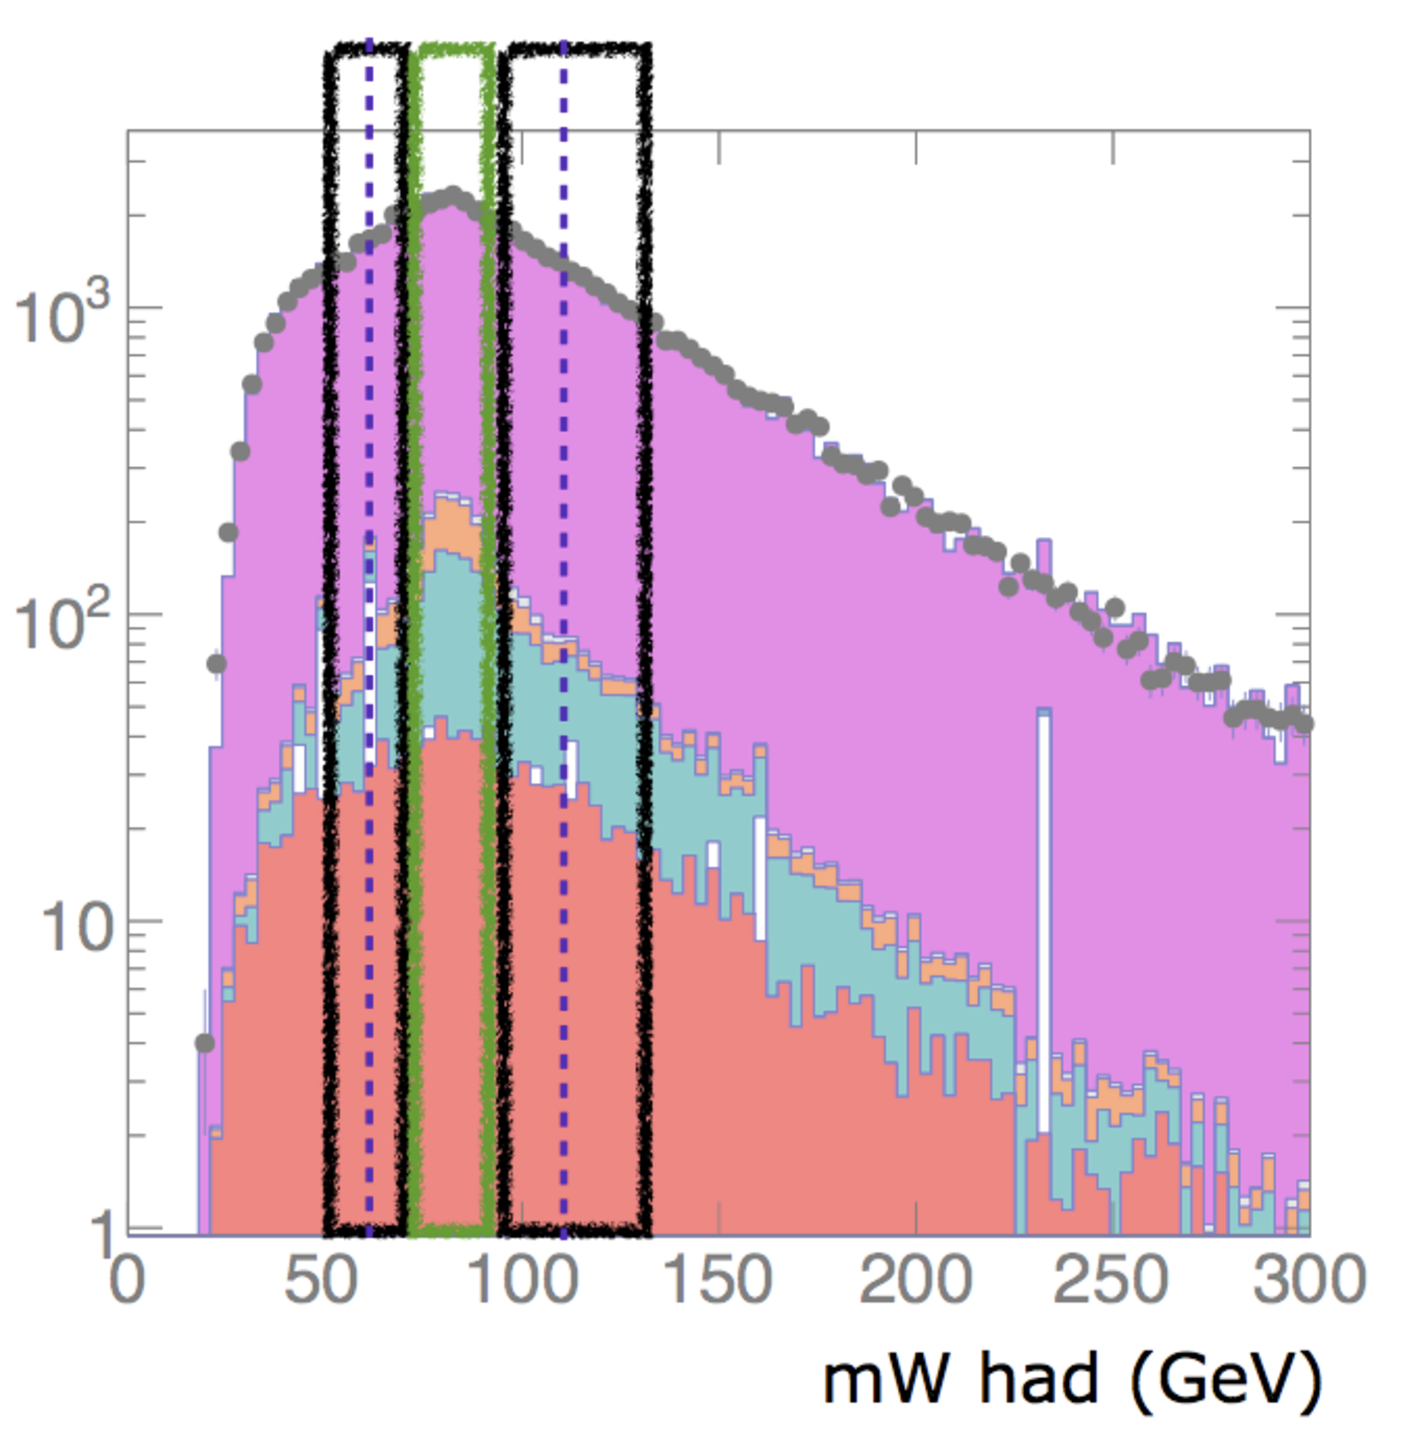
\includegraphics[width=0.45\textwidth]{plots/sideband/sbSidebands.pdf}
    \caption{Pictorical representation of the sideband regions definition (black boxes) 
             and of the signal region (green box),
             superimposed to the two-body invariant mass shape.
             Further division of sidebands are outlined with dashed lines.}
    \label{fig:sbSidebands}
  \end{center}
\end{figure}
%
Each sideband is further divided into two subregions, 
of comparable events population.
The limits are 57~GeV for the low $m_{jj}$ sideband
and 107~GeV for the high $m_{jj}$ one,
as outiled with dashed lines in Figure~\ref{fig:sbSidebands}.

%binning

% ---- ---- ---- ---- ---- ---- ---- ---- ---- ---- ---- ---- ---- ---- ---- ---- ---- ---- ---- ---- ---- ---- ----


\subsection{The extrapolation factor}

The extrapolation factor $\alpha(m_{WW})$ 
is calculated as the ratio of the $m_{\ell\nu{}jj}$ spectrum
between sidebands and signal region.
In this way, 
the background evaluation in the signal region, on data, 
will be:
\begin{equation}
N_{bkg}(m_{WW})~=~N_{sb}(m_{WW})~\times~\frac{N_{bkg}^{MC}(m_{WW})}{N_{sb}^{MC}(m_{WW})}~=~N_{sb}(m_{WW})~\times~\alpha(m_{WW})~.
\label{eq:sbExtrapolation}
\end{equation}

The distributions used to build the ratio are reported in Figure~\ref{fig:sbNumDen},
where the composition in terms of different samples is shown
for the numerator (on the left)
and for the denominator (on the right).
%
\begin{figure}[htb]
  \begin{center}
    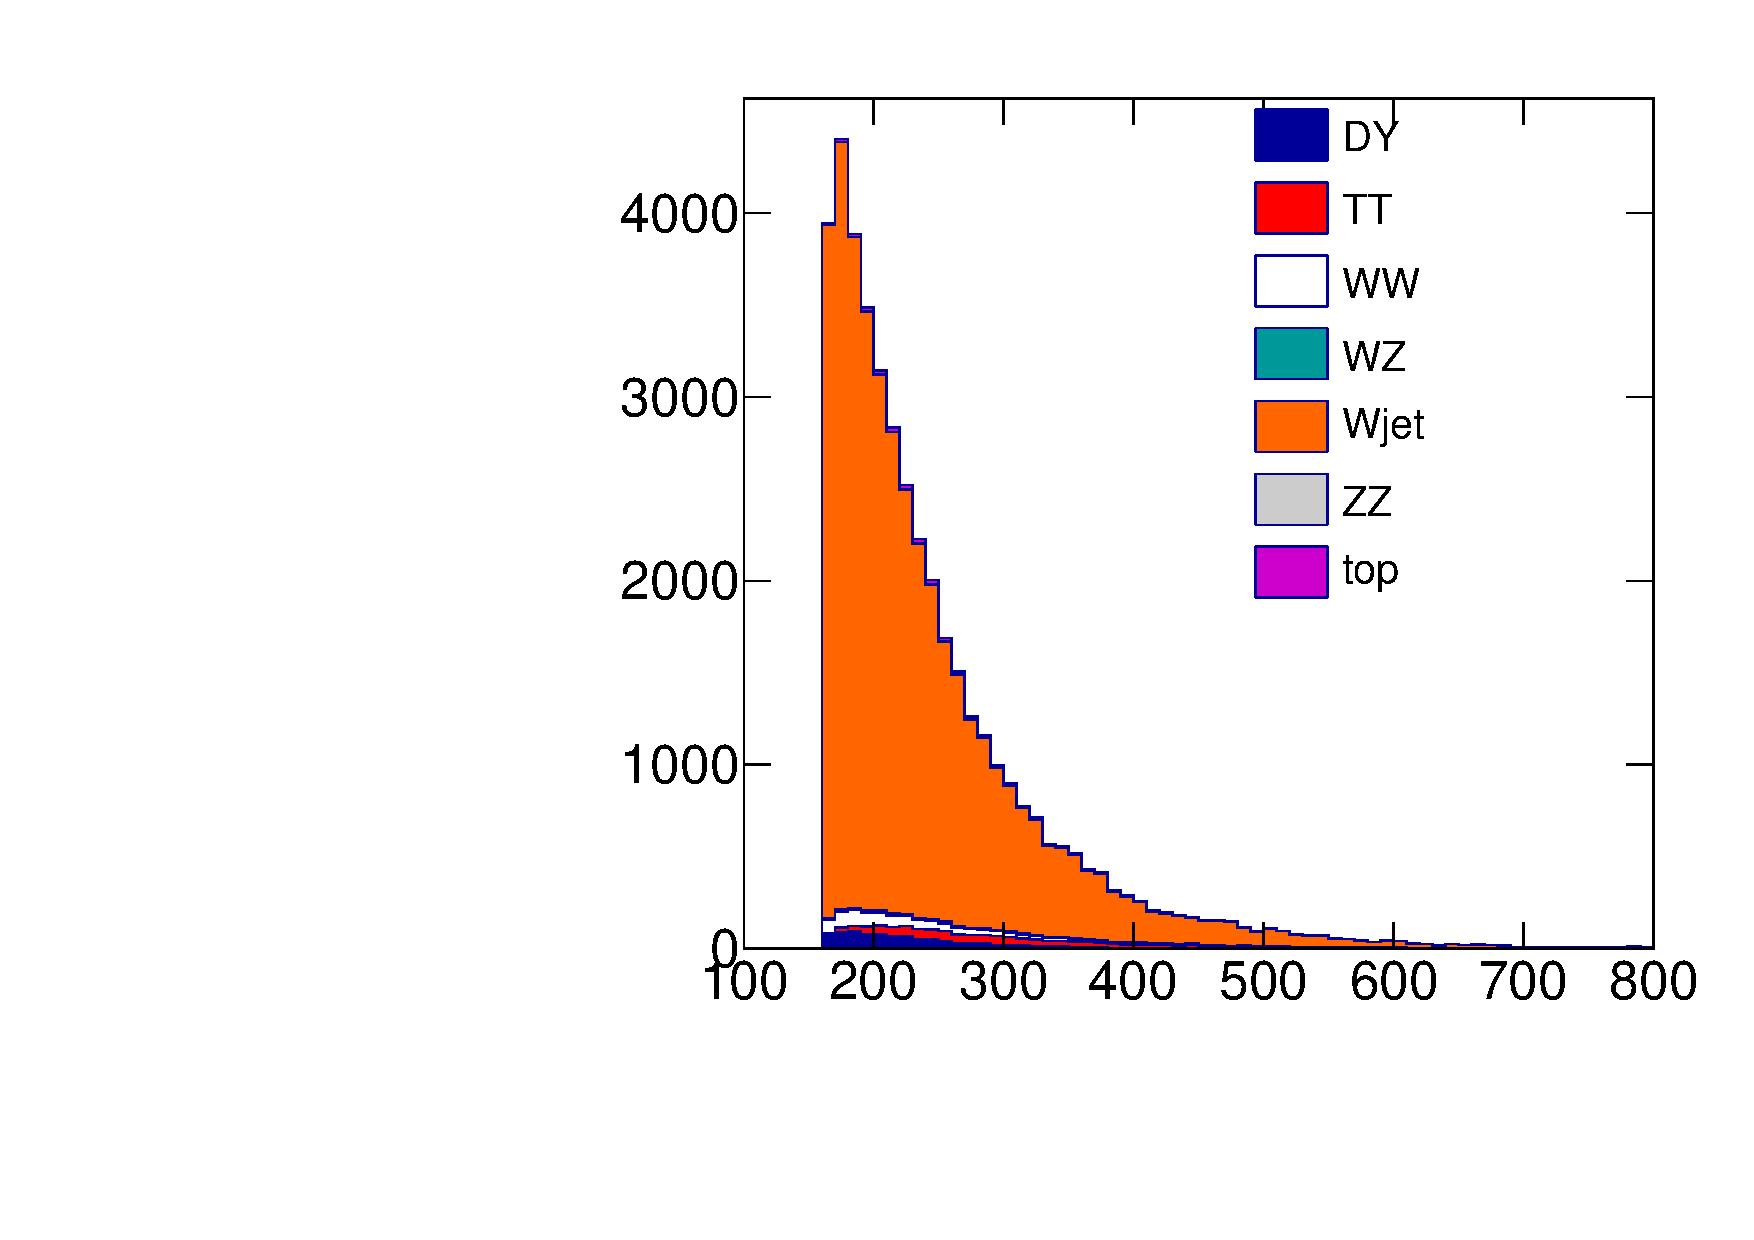
\includegraphics[width=0.45\textwidth]{plots/sideband/sbNumMCComposition.pdf}
    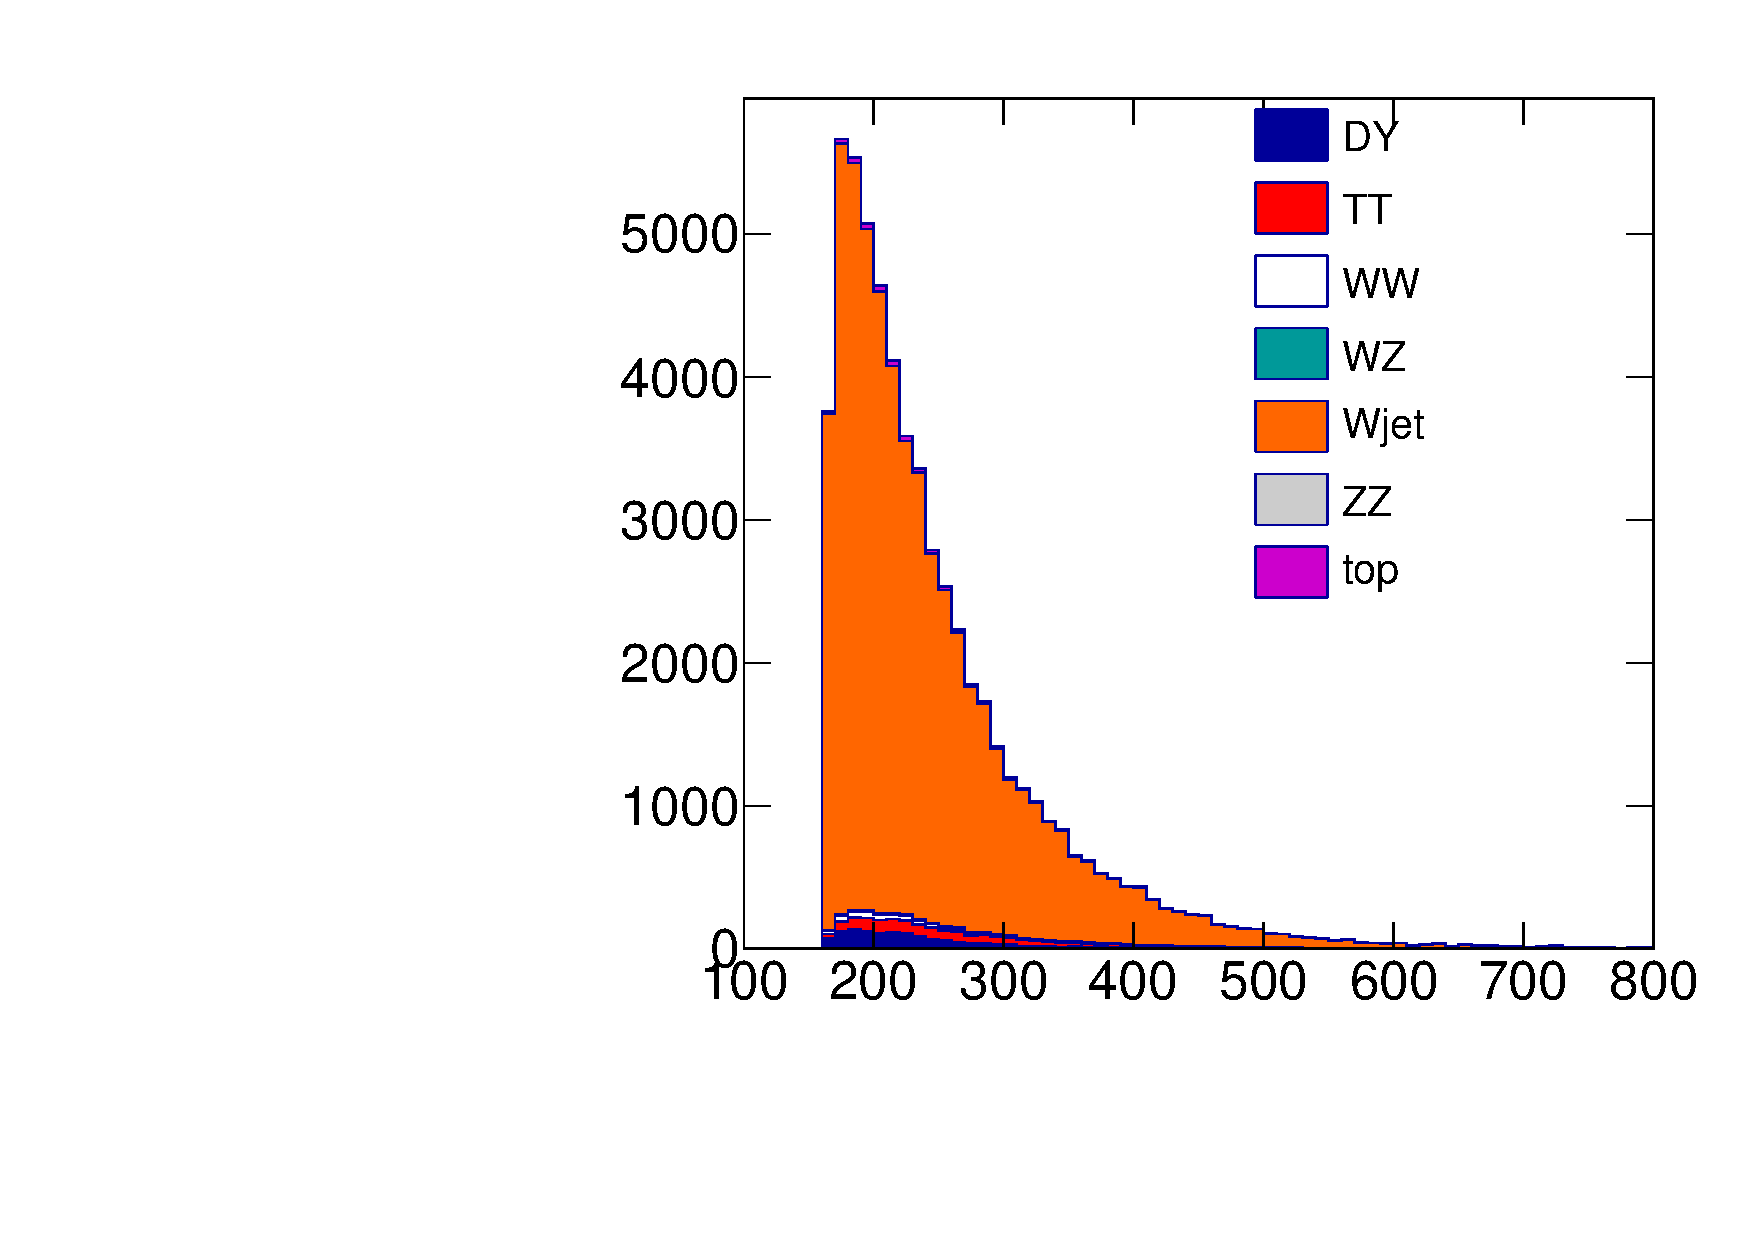
\includegraphics[width=0.45\textwidth]{plots/sideband/sbDenMCComposition.pdf}
    \caption{The distributions used to build the $\alpha(m_{WW})$ extrapolation factor,
             where the composition in terms of different samples is shown
             for the numerator (on the left)
             and for the denominator (on the right).}
    \label{fig:sbNumDen}
  \end{center}
\end{figure}
%
The two distributions are smoothed by means of a double exponential fit 
(the function is described in Equation~\ref{eq:fitDoubleExp})
from 200~GeV onwards, 
and the $\alpha(m_{WW})$ factor is calculated as the ratio of the fitting functions
with the same binning of the initial histograms.
The uncertainty on the correction factor is obtained by propagating the uncertainties
on the fitted functions, 
which come from the uncertainty bands derived from the uncertainties on the fitting parameters, 
treated with the proper correlations.
Figure~\ref{fig:sbNumDenFits} show the fits to the numerator (on the left) and denominator (on the right),
with the fitting function superimposed to the total simulated shapes,
and with the uncertainty bands in grey.
%
\begin{figure}[htb]
  \begin{center}
    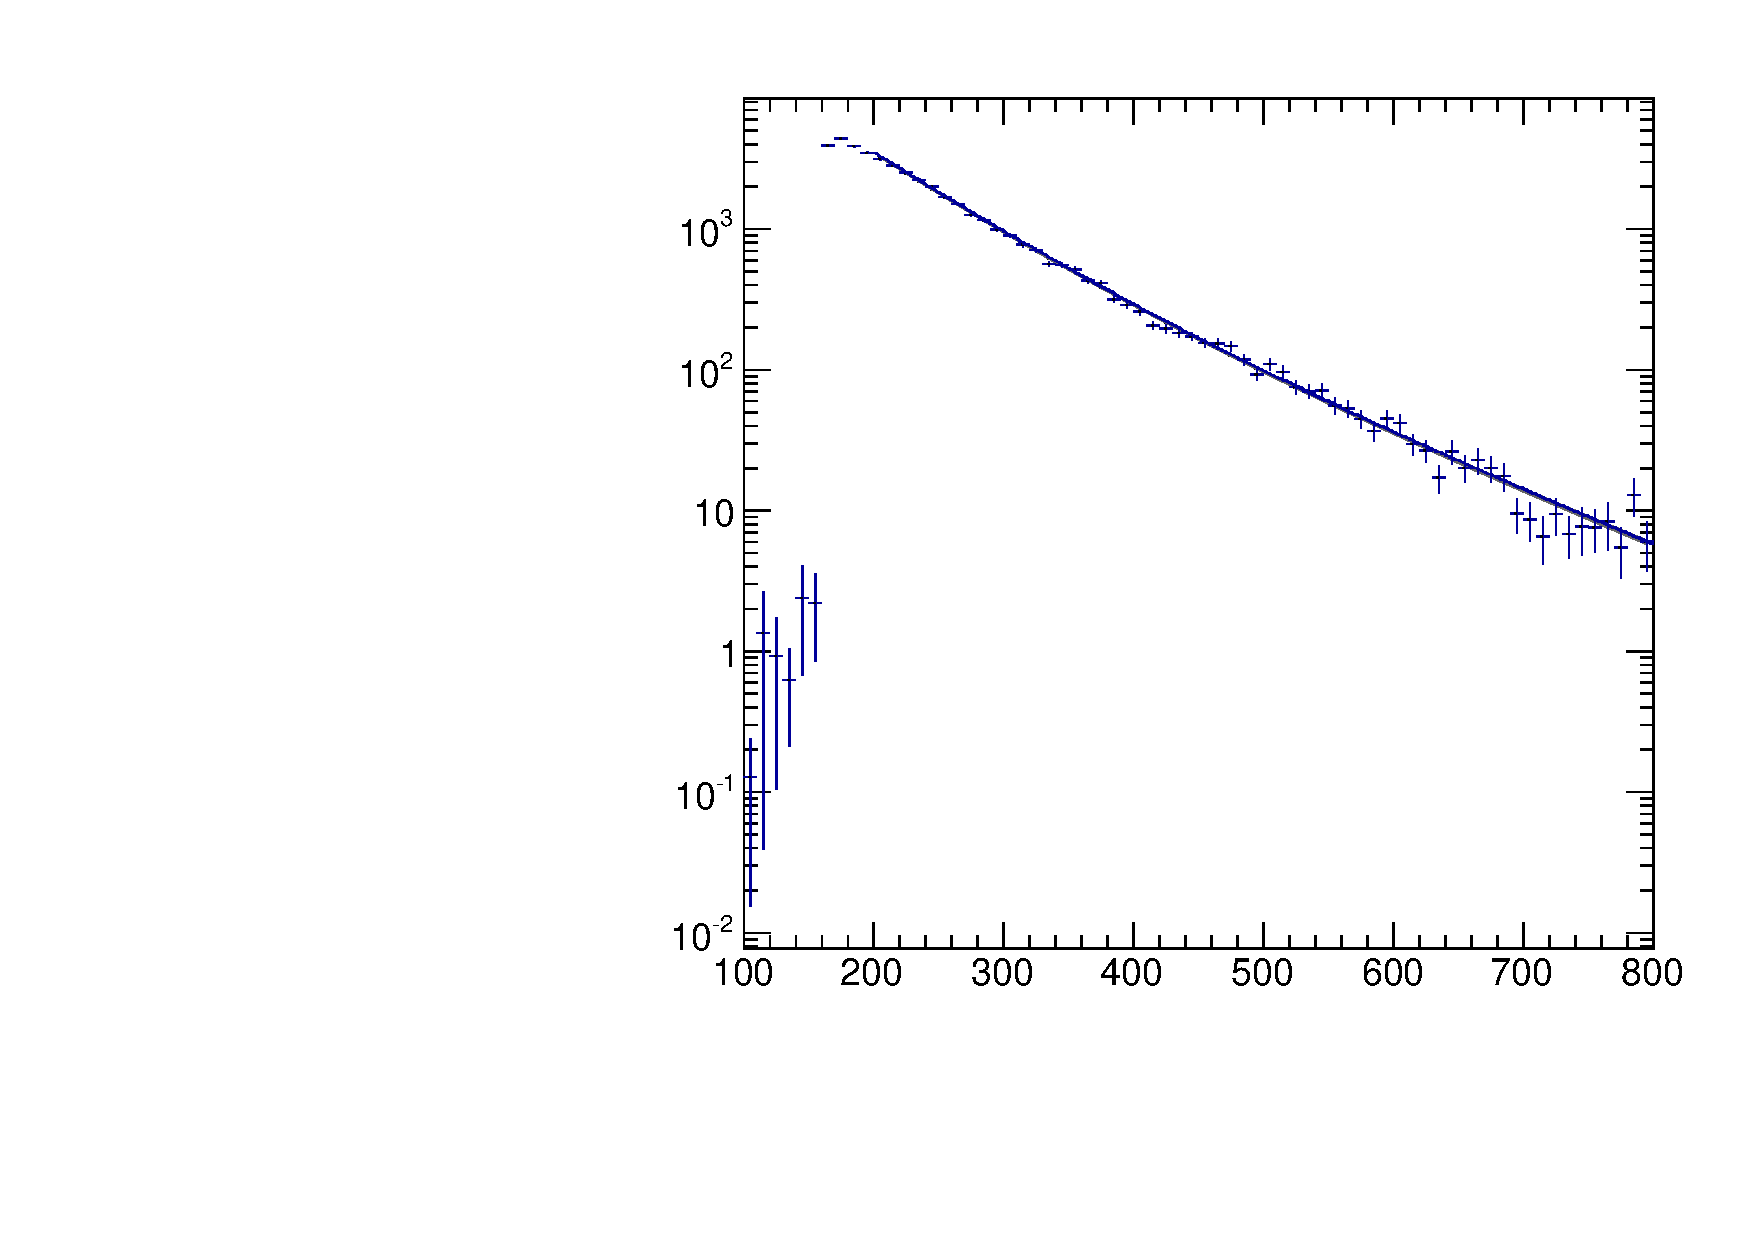
\includegraphics[width=0.45\textwidth]{plots/sideband/sbNumMCFit.pdf}
    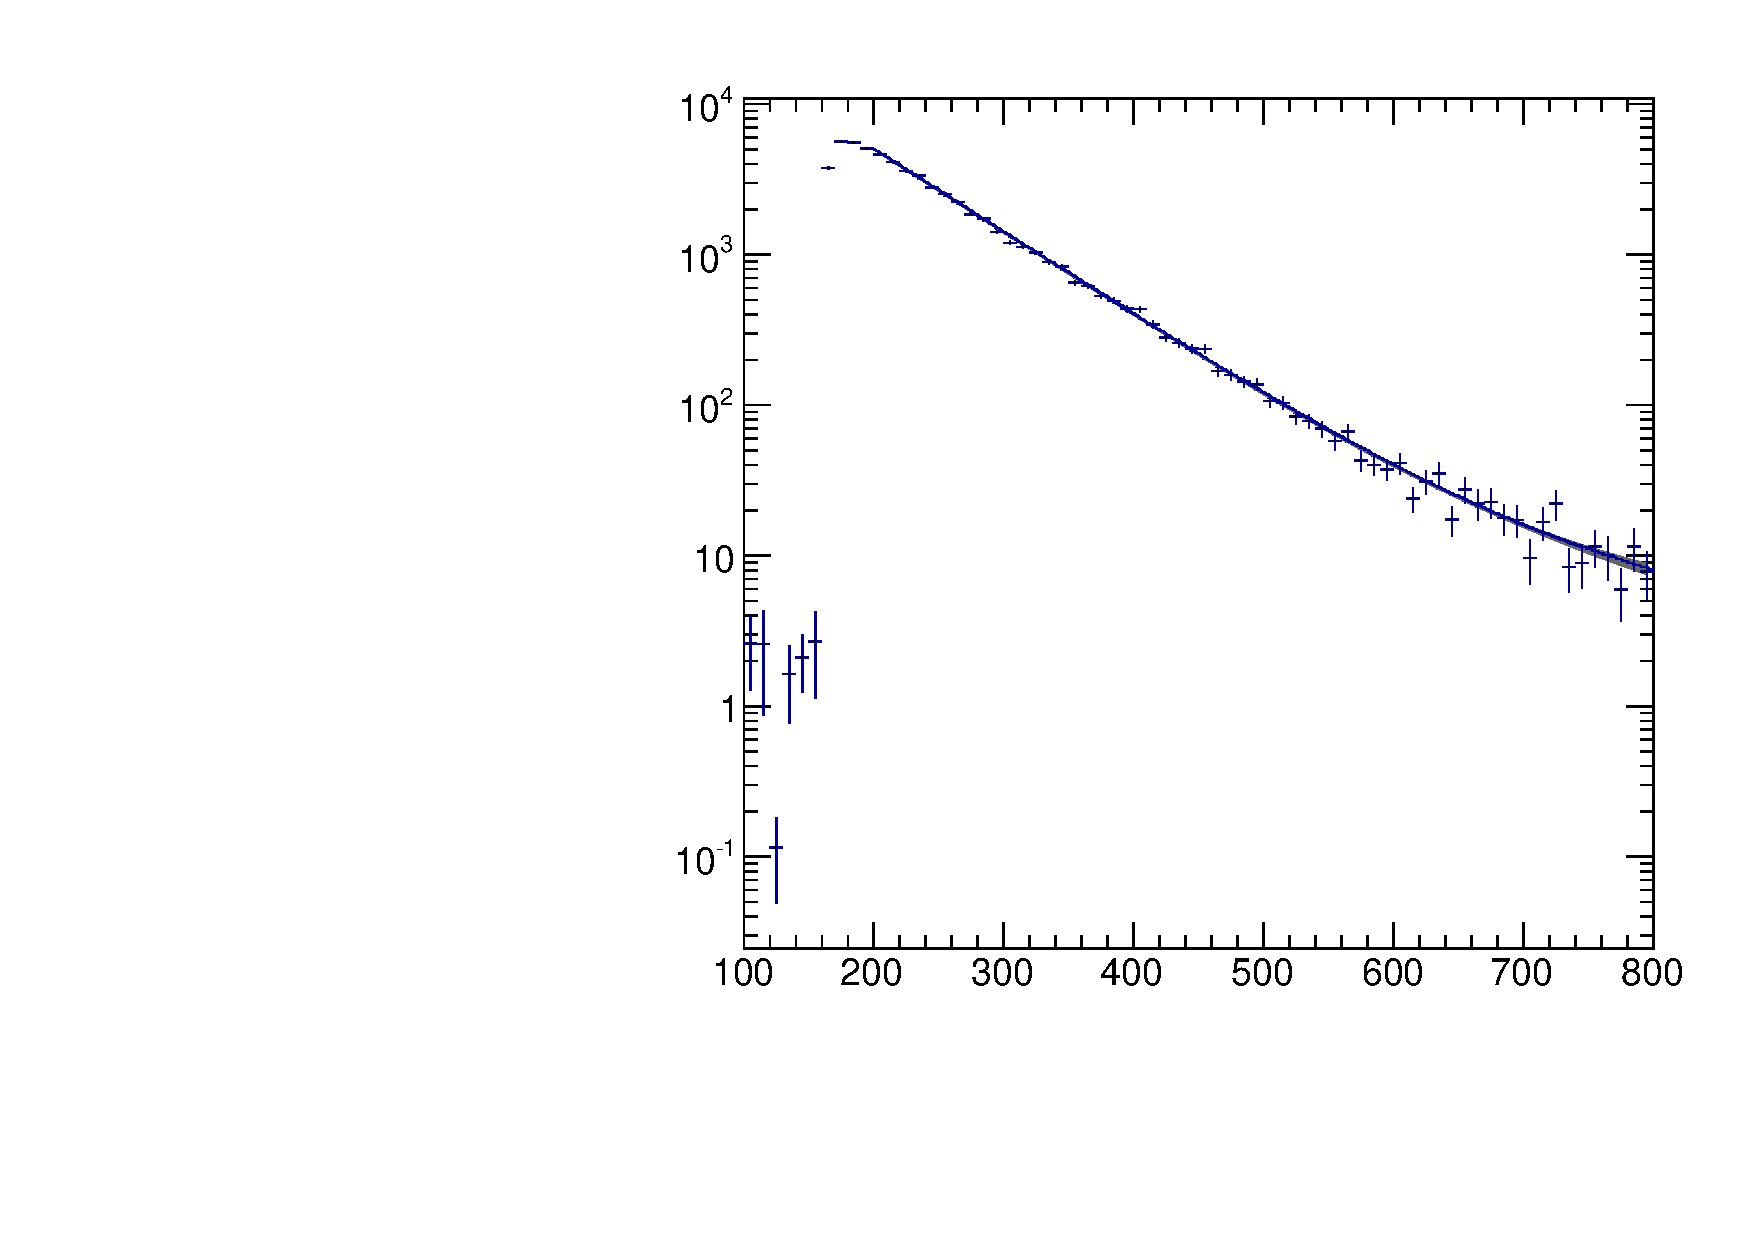
\includegraphics[width=0.45\textwidth]{plots/sideband/sbDenMCFit.pdf}
    \caption{The fits to the simulation numerator (on the left) and denominator (on the right),
             with the fitting function superimposed to the total simulated shapes,
             and with the uncertainty bands in grey.}
    \label{fig:sbNumDenFits}
  \end{center}
\end{figure}
%
Figure~\ref{fig:sbAlpha} shows the correction factor,
obtained as ratio between the two fitting functions.
The yellow band shows the obtained uncertainty, 
while the markers show the ratio one obtains by dividing the two histograms of Figure~\ref{fig:sbNumDen}.
%
\begin{figure}[htb]
  \begin{center}
    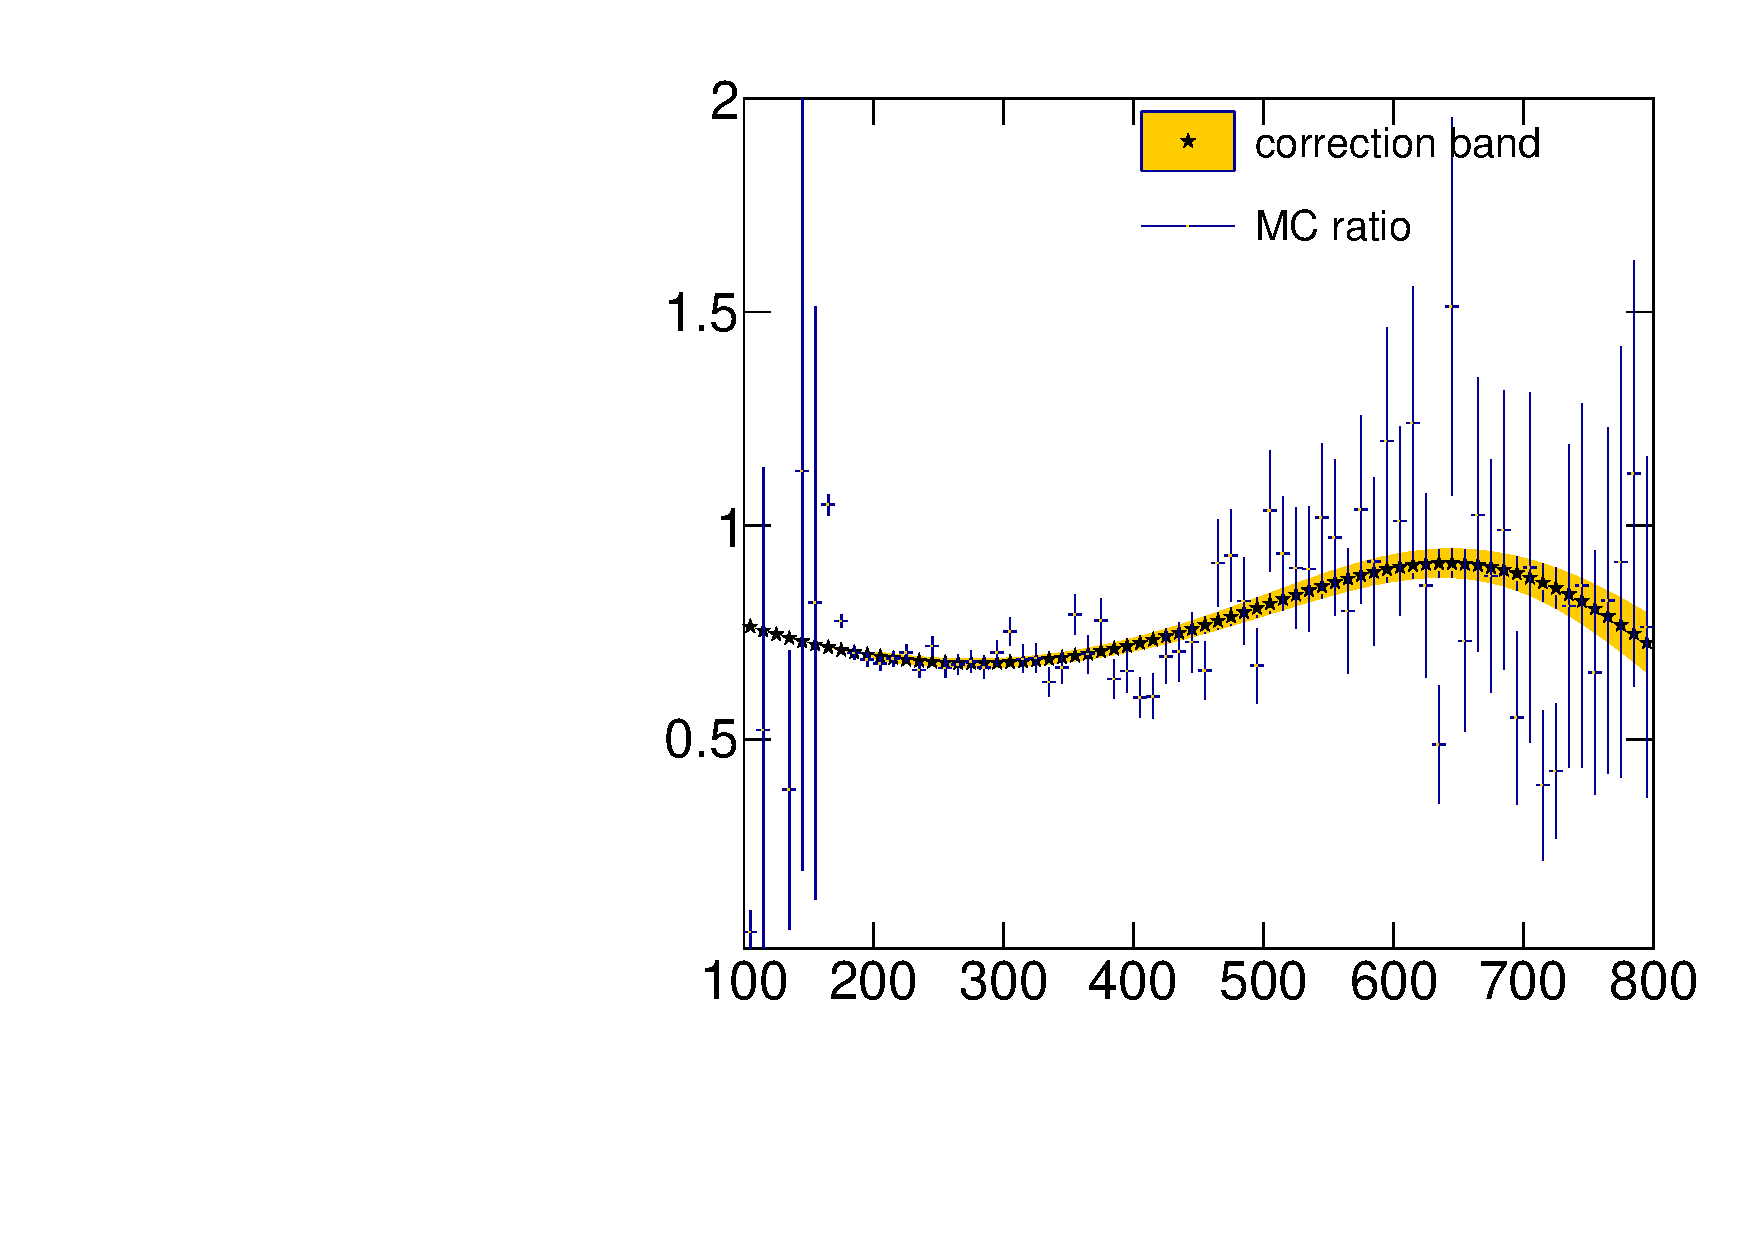
\includegraphics[width=0.45\textwidth]{plots/sideband/sbAlpha.pdf}
    \caption{The $\alpha(m_{WW})$ correction factor,
             obtained as ratio between the two fitting functions of Figure~\ref{fig:sbNumDenFits}.
             The yellow band shows the obtained uncertainty, 
             while the markers show the ratio one obtains 
             by dividing the two histograms of Figure~\ref{fig:sbNumDen}.}
    \label{fig:sbAlpha}
  \end{center}
\end{figure}
%


% ---- ---- ---- ---- ---- ---- ---- ---- ---- ---- ---- ---- ---- ---- ---- ---- ---- ---- ---- ---- ---- ---- ----


\subsection{Analysis closure test}

To check that the fits applied in the $\alpha(m_{WW})$ do not introduce biases, 
a closure test is performed on the simulation itself.
Figure~\ref{fig:sbMCClosure} shows the comparison between the expected background in the signal region (black markers)
with respect to the extrapolated one from the sidebands (yellow band), 
as a function of $m_{\ell\nu{}jj}$.
The error bars on the expected signal is the statistical uncertainty,
while the yellow band is the uncertainty due to the one on alpha and the statistics in the sidebands.
On the left, 
the distributions are superimposed,
while on the right the pull plot is shown.
%
\begin{figure}[htb]
  \begin{center}
    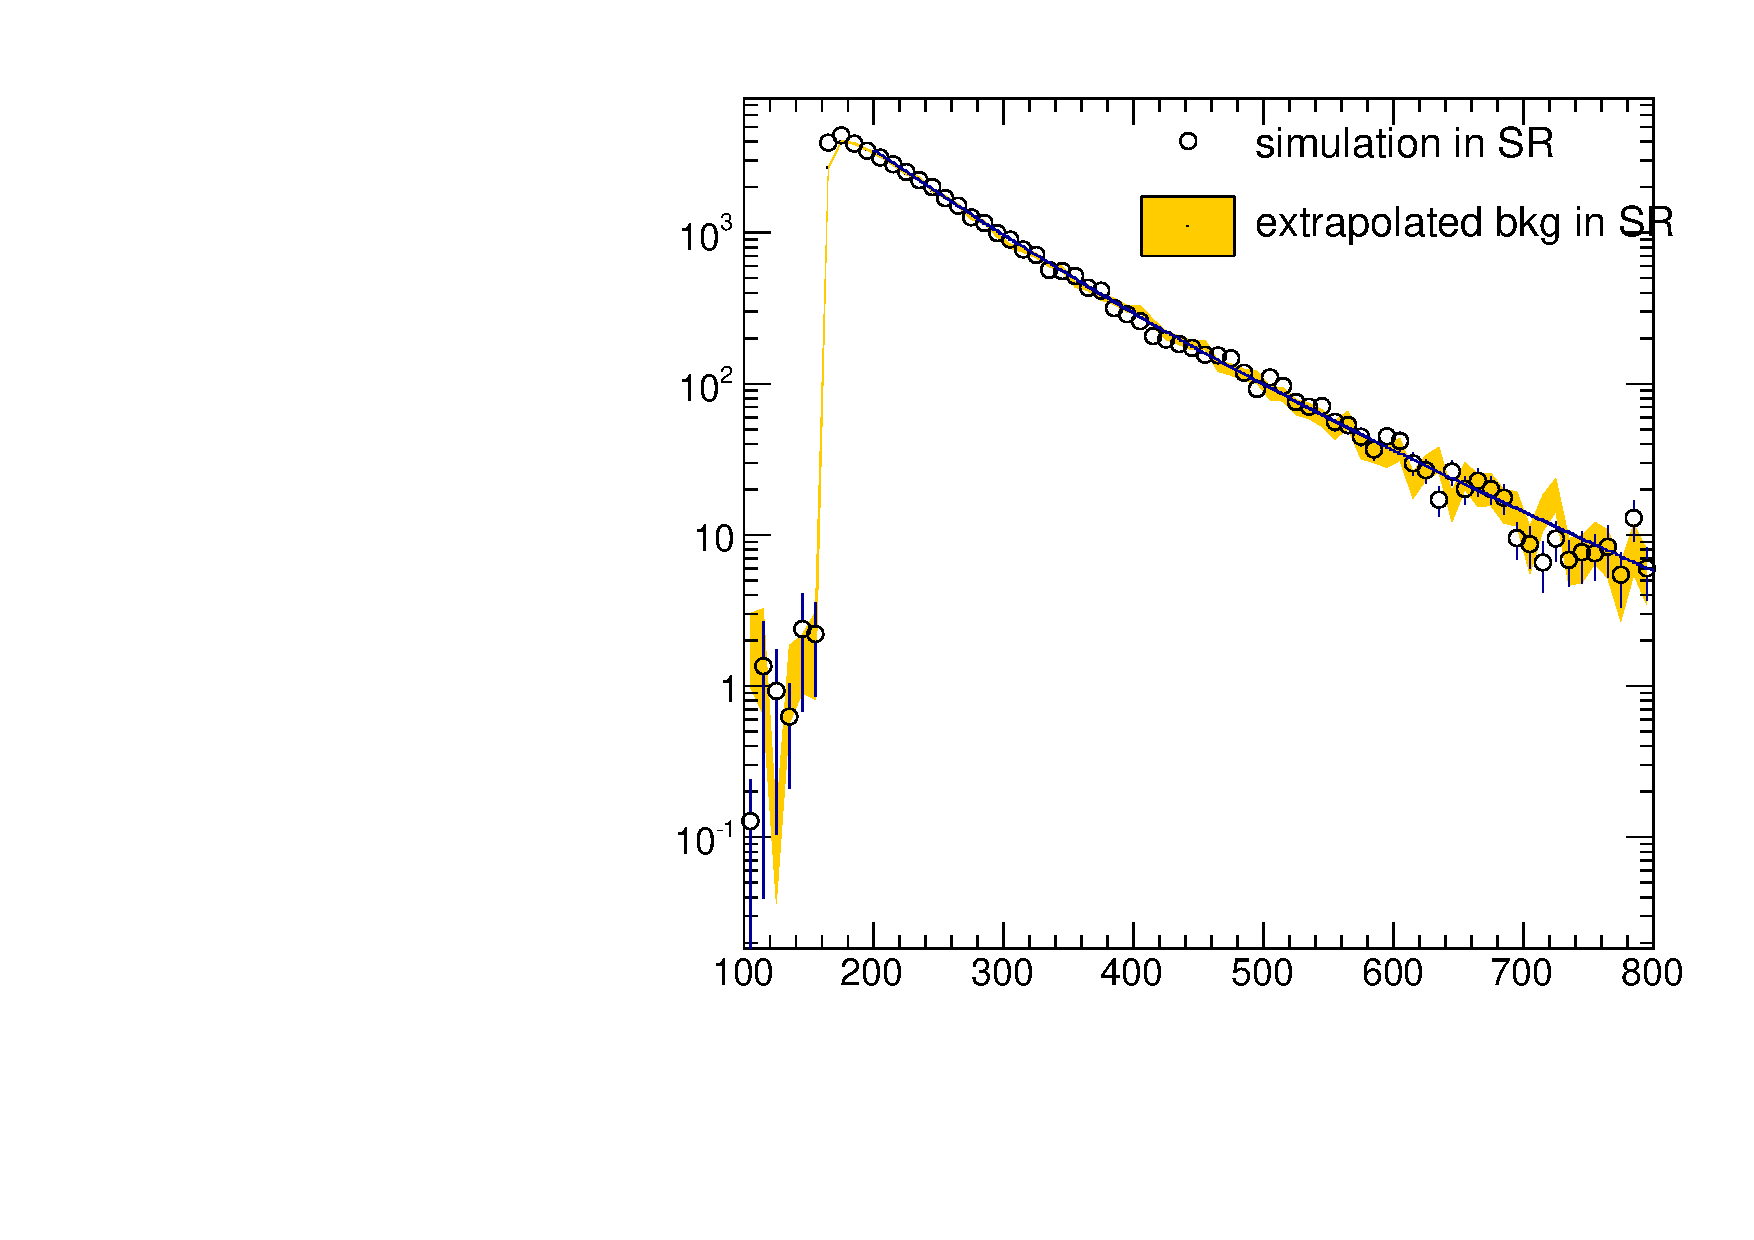
\includegraphics[width=0.45\textwidth]{plots/sideband/sbMCClosureDistrib.pdf}
    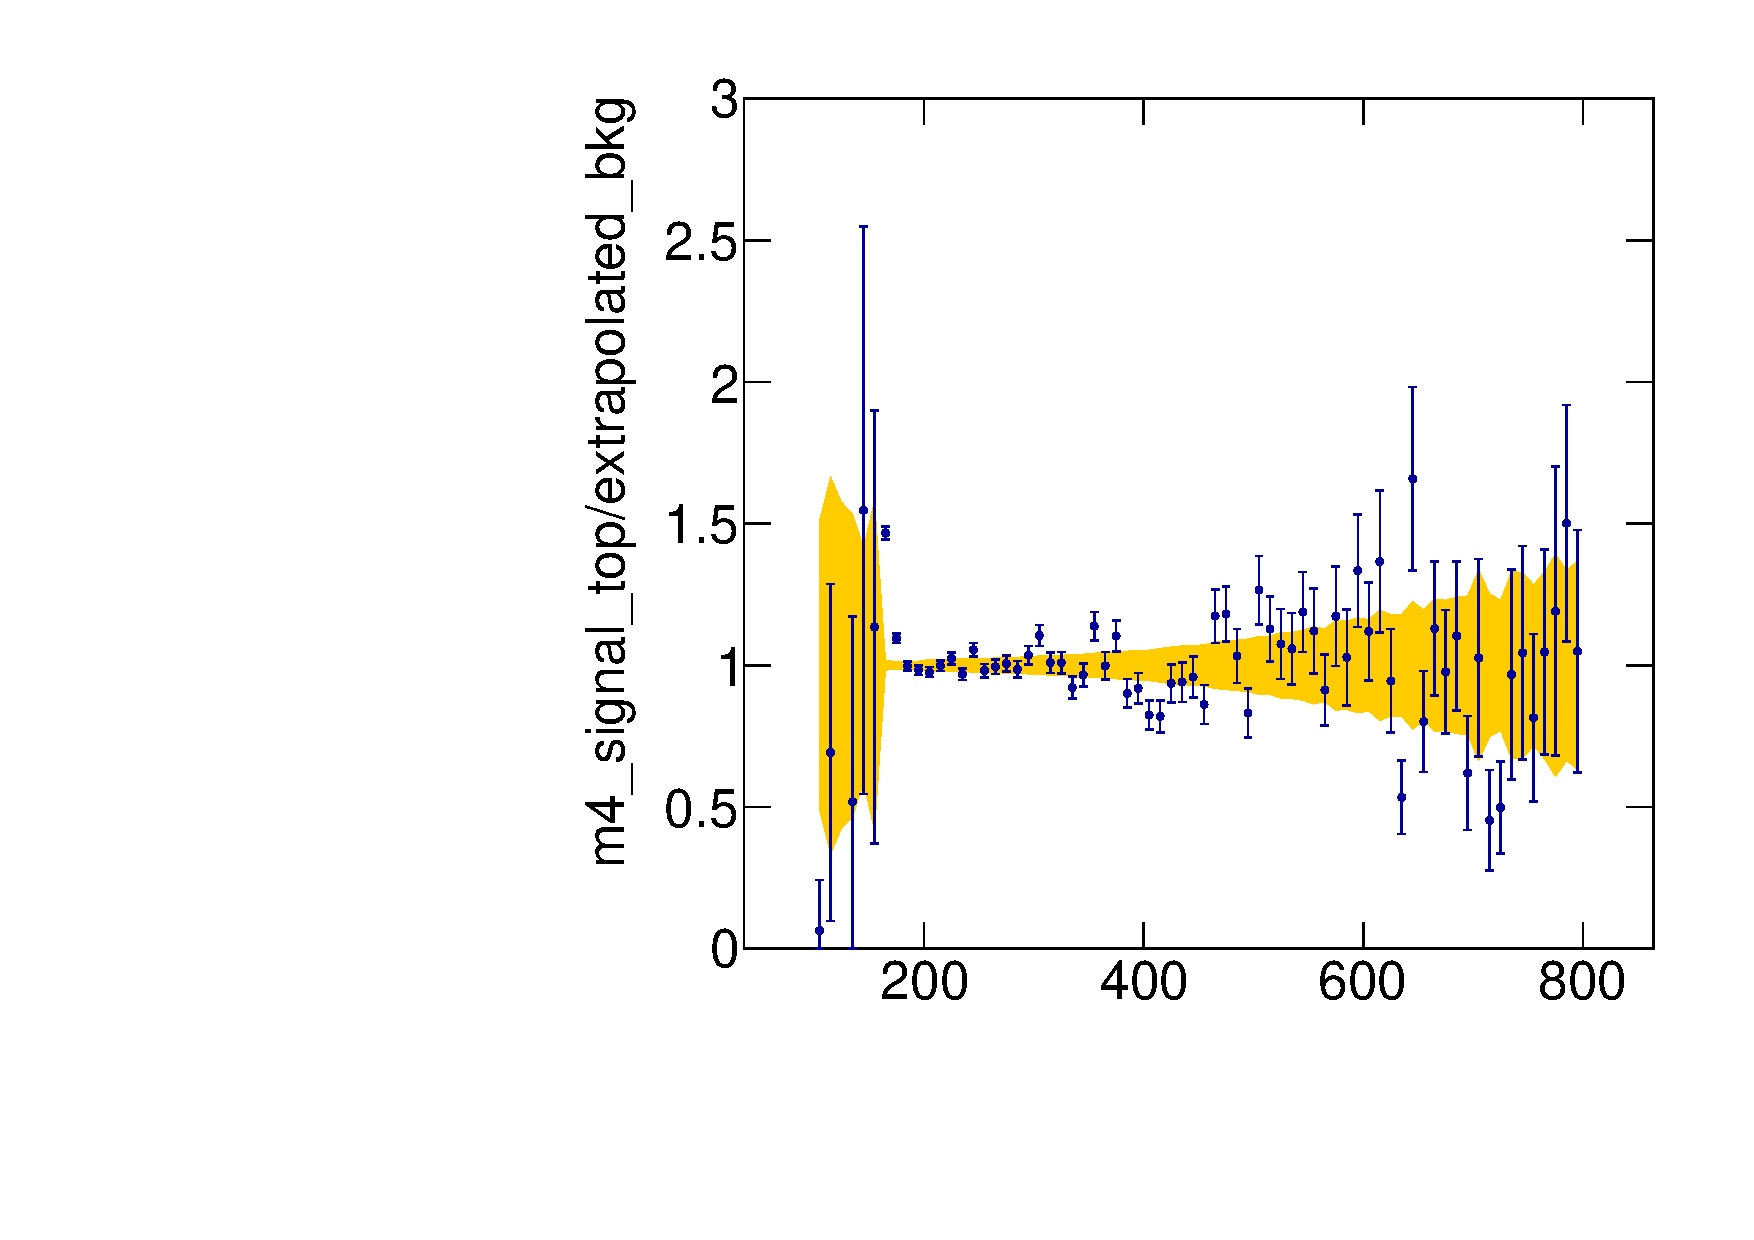
\includegraphics[width=0.45\textwidth]{plots/sideband/sbMCClosurePull.pdf}
    \caption{The comparison between the expected background in the signal region (black markers)
             with respect to the extrapolated one from the sidebands (yellow band), 
             as a function of $m_{\ell\nu{}jj}$.
             The error bars on the expected signal is the statistical uncertainty,
             while the yellow band is the uncertainty due to the one on alpha and the statistics in the sidebands.
             On the left, 
             the distributions are superimposed,
             while on the right the pull plot is shown.}
    \label{fig:sbMCClosure}
  \end{center}
\end{figure}
%
Since the fit in the extrapolation factor is performed from 200~GeV onwards, 
the comparison is meaningful only above the threshold.
As can be seen, so systematic effects are visible in the plot.
\textbf{FIXME need to make the pull distibution, not only the pull trend}


% ---- ---- ---- ---- ---- ---- ---- ---- ---- ---- ---- ---- ---- ---- ---- ---- ---- ---- ---- ---- ---- ---- ----


\subsection{Extrapolation test on sidebands}

To verify the predictive power of the technique on data,
the side-bands have been divided into two sub-regions each, 
as sketched in Figure~\ref{fig:sbSidebands}.
The division is such, to preserve about the same number of events in each sub-region.
The background extrapolation technique is then applied
to predict the background shape in the two regions closest to the signal region,
starting from the two distant ones.
Figure~\ref{fig:sbsbAlphaSBtest} shows the correction factor, 
calculated for this specific configuration.
The markers show the value used,
while the yellow band is the error assigned to it.
%
\begin{figure}[htb]
  \begin{center}
    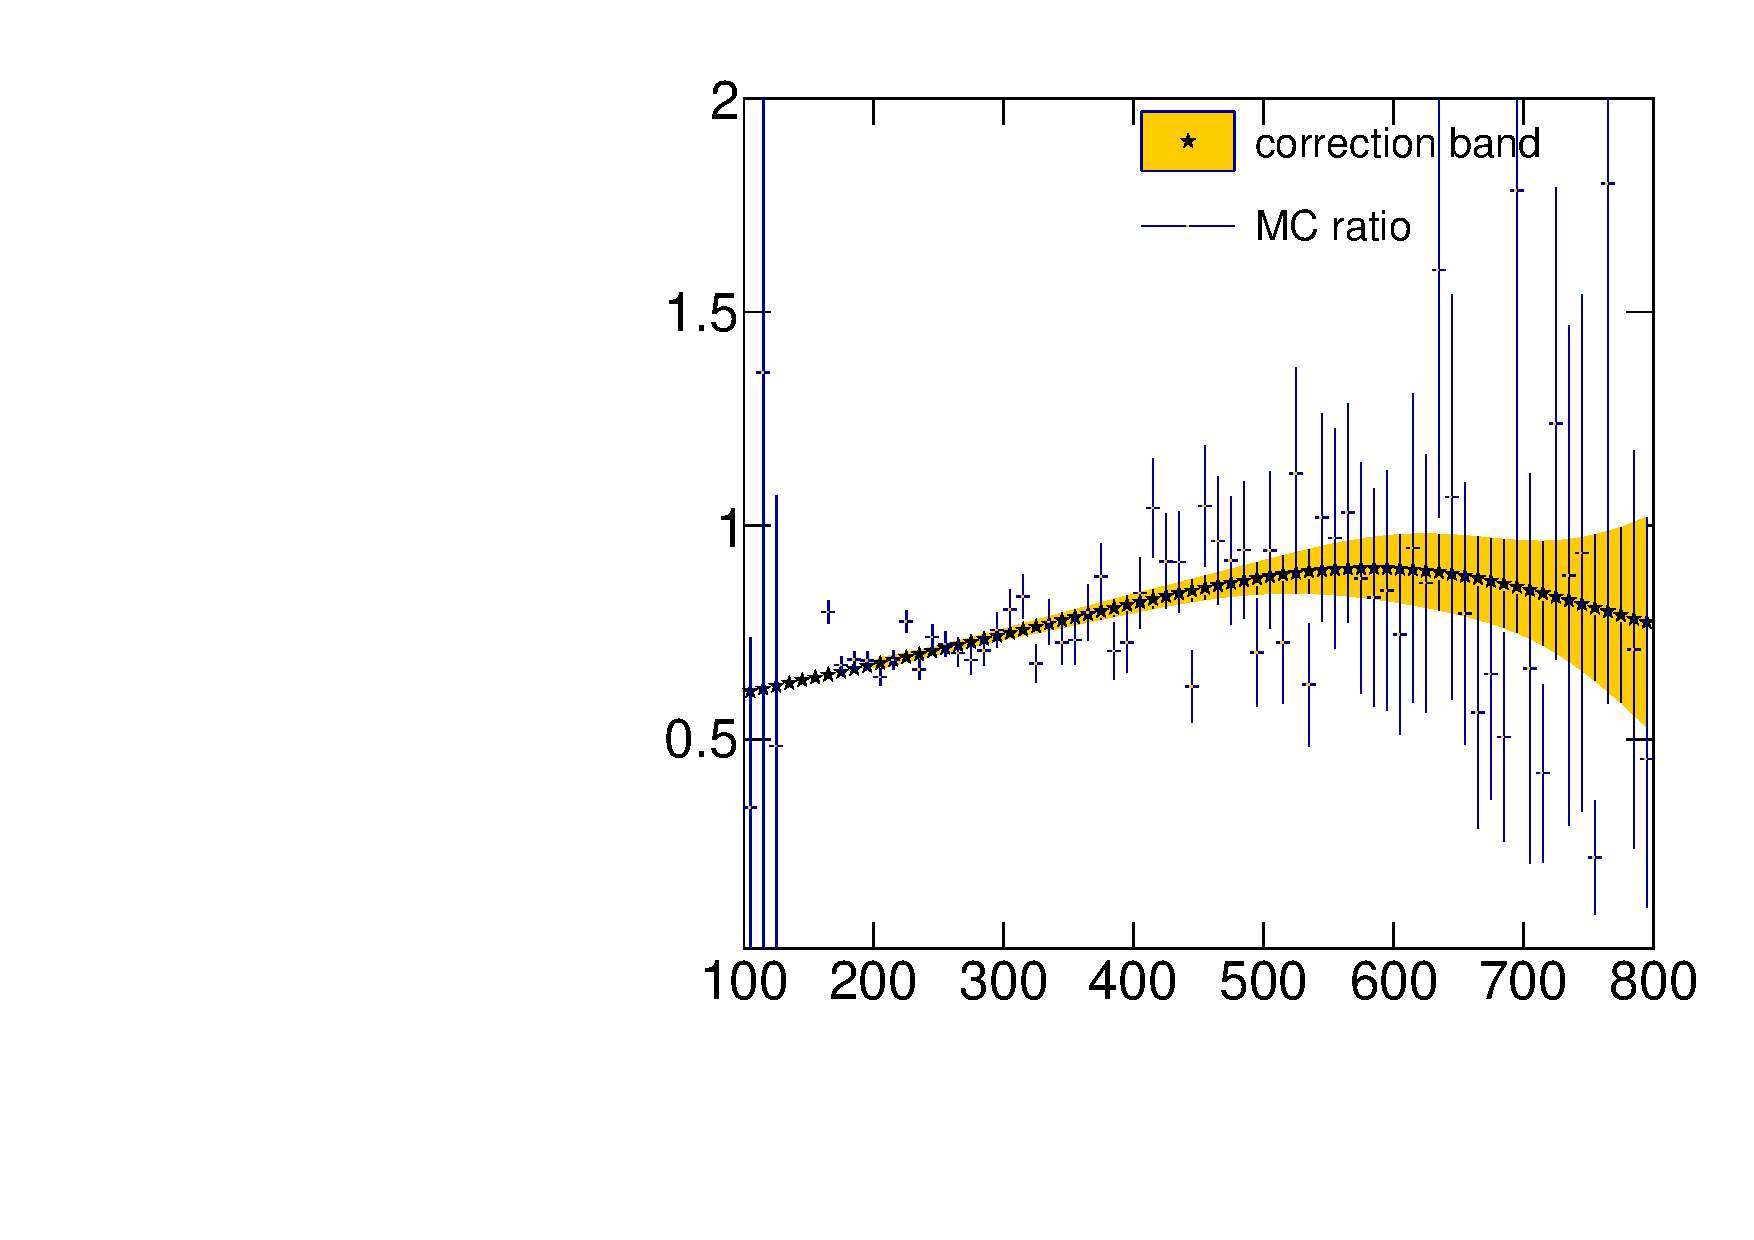
\includegraphics[width=0.45\textwidth]{plots/sideband/sbsbAlphaSBtest.pdf}
    \caption{The $\alpha(m_{WW})$ correction factor,
             calculated for the extrapolation test configuration.
             The yellow band shows the obtained uncertainty, 
             while the markers show the ratio one obtains 
             by dividing the two histograms of the simulation without any regularizations applied.}
    \label{fig:sbsbAlphaSBtest}
  \end{center}
\end{figure}
%
For comparison,
the correction factor that one would obtain by simply dividing the two histograms
obtained from simulation before the fit, 
is reported in blue.
Figure~\ref{fig:sbBkgSBtest} shows the number of events in the regions closest to the signal region
(black dots) and the preodicted ones from the external sidebands (yellow band).
%
\begin{figure}[htb]
  \begin{center}
    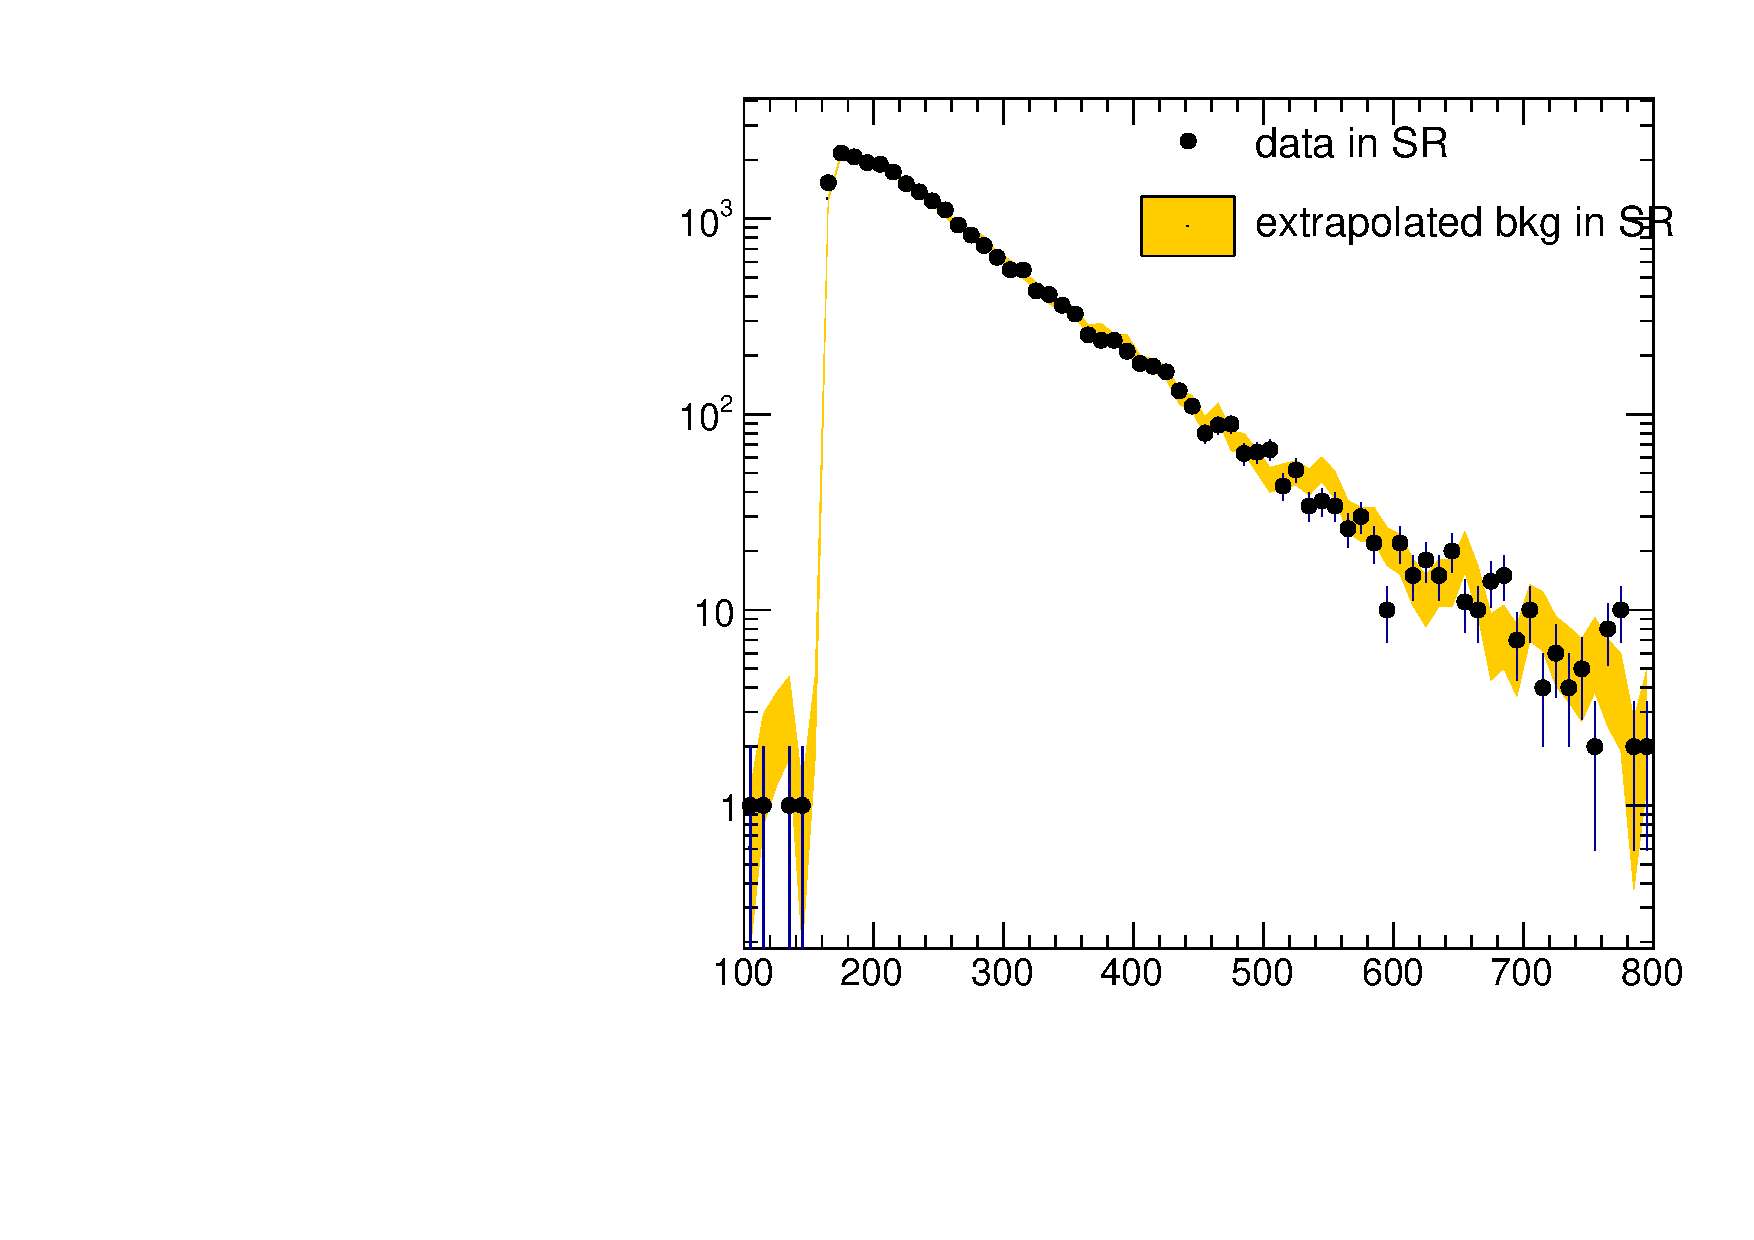
\includegraphics[width=0.45\textwidth]{plots/sideband/sbBkgSBtest.pdf}
    \caption{The four-body invariant mass spectrum in the internal sidebands (black dots),
             superimposed to its estimate derived from the external sidebands (yellow band).}
    \label{fig:sbBkgSBtest}
  \end{center}
\end{figure}
%
Figure~\ref{fig:sbBkgSBtestPull} shows the trend of the ratio between the two distributions (left),
and the pull plot, 
calculated in the regularization fit range,
between the two distributions.
%
\begin{figure}[htb]
  \begin{center}
    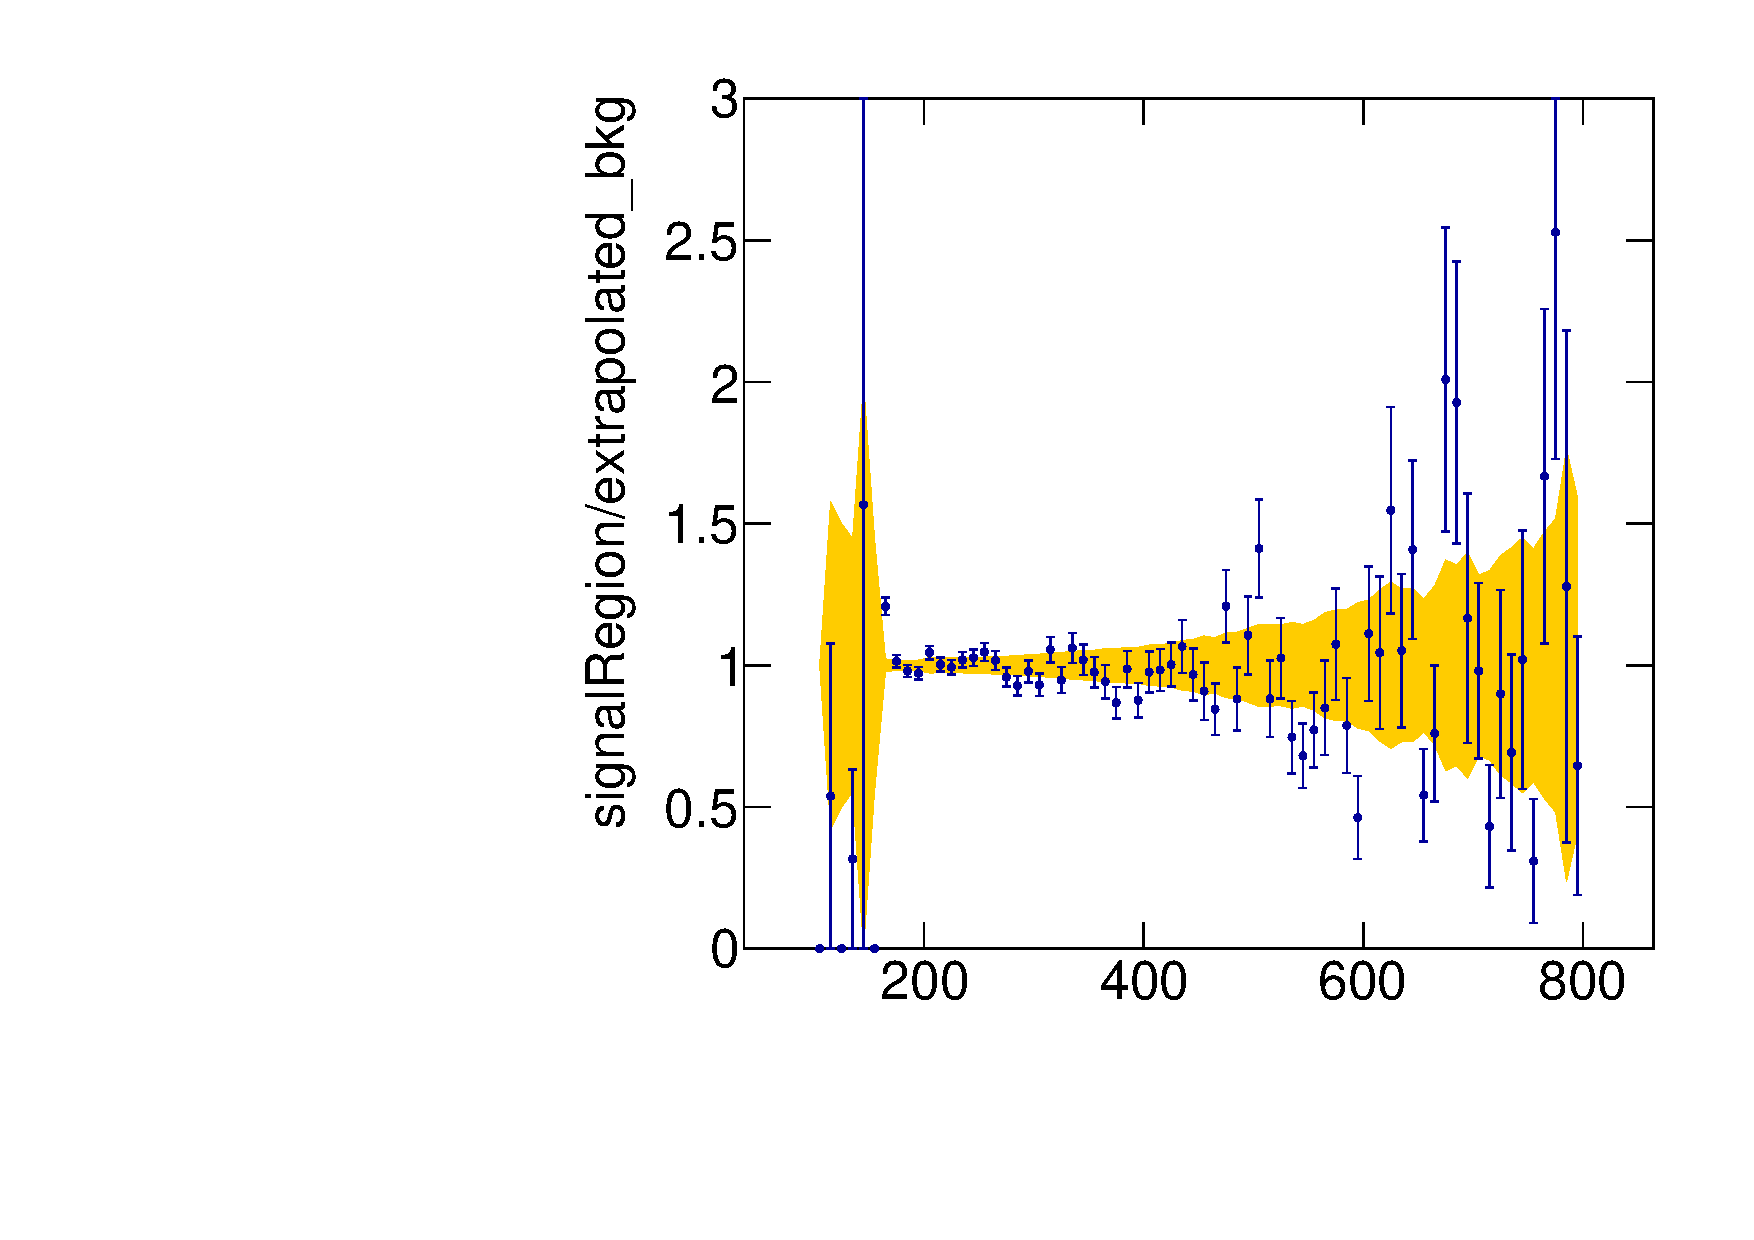
\includegraphics[width=0.45\textwidth]{plots/sideband/sbBkgSBtestPullTrend.pdf}
    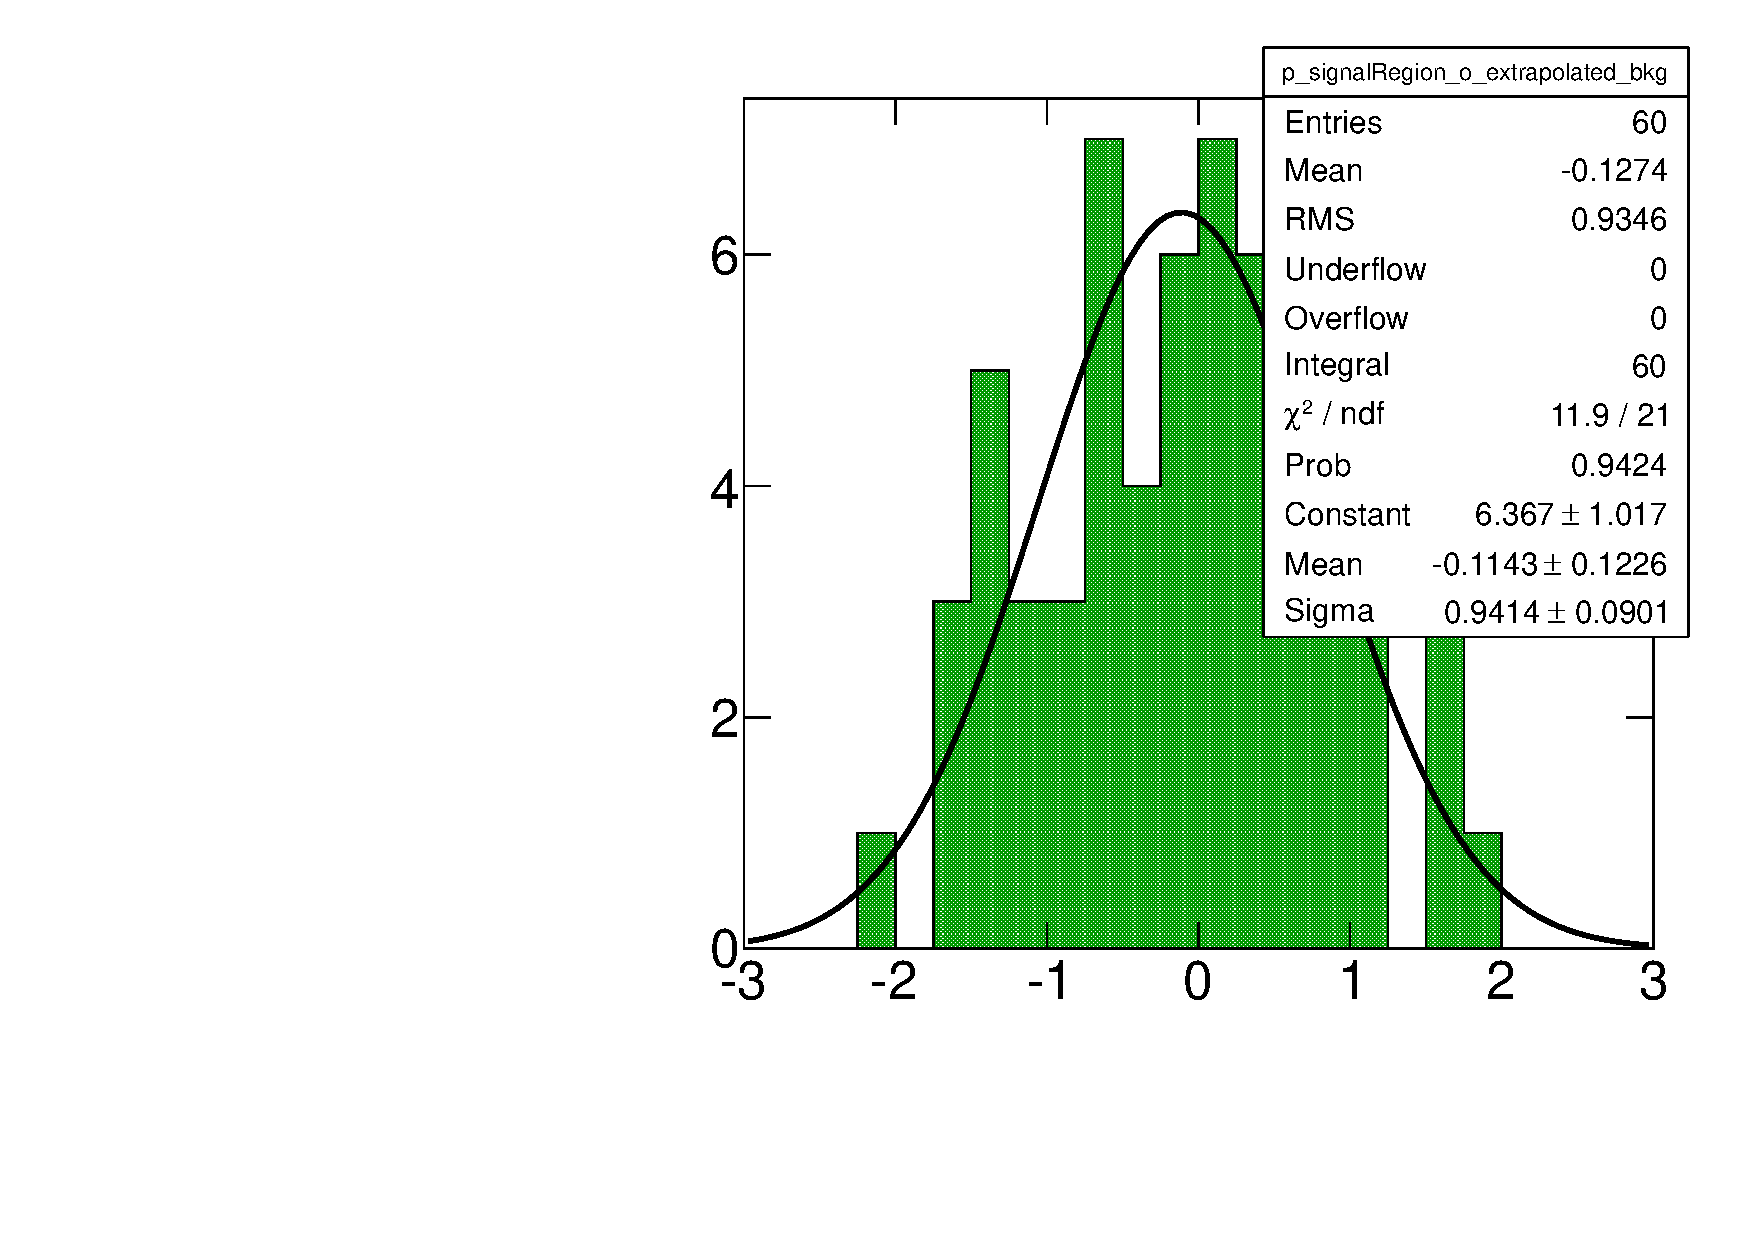
\includegraphics[width=0.45\textwidth]{plots/sideband/sbBkgSBtestPullPlot.pdf}
    \caption{The trend of the ratio (left)
             and the pull plot
             calculated in the regularization fit range,
             between the two distributions of Figure~\ref{fig:sbBkgSBtest}.}
    \label{fig:sbBkgSBtest}
  \end{center}
\end{figure}
%
The two results are compatible within the uncertainty.


% ---- ---- ---- ---- ---- ---- ---- ---- ---- ---- ---- ---- ---- ---- ---- ---- ---- ---- ---- ---- ---- ---- ----


\subsection{Signal injection}

A possible effect due to the signal contamination in the sideband regions
has been investigated by injecting signal in the closure test,
for the hypothesis of a 350~GeV Higgs.
The difference between the background extrapolated in this case, 
to the one obtained without the signal injection, 
is compared to the expected signal and to the error band of the signal extrapolation.
Figure~\ref{fig:sbSigInjection} shows this test,
where the yellow band represents the error in the extrapolation without signal injection, 
the blue crosses show the difference of the backgrounds extarpolated in the two cases,
and the black line is the expected number of signal events in case of Higgs presence.
%
\begin{figure}[htb]
  \begin{center}
    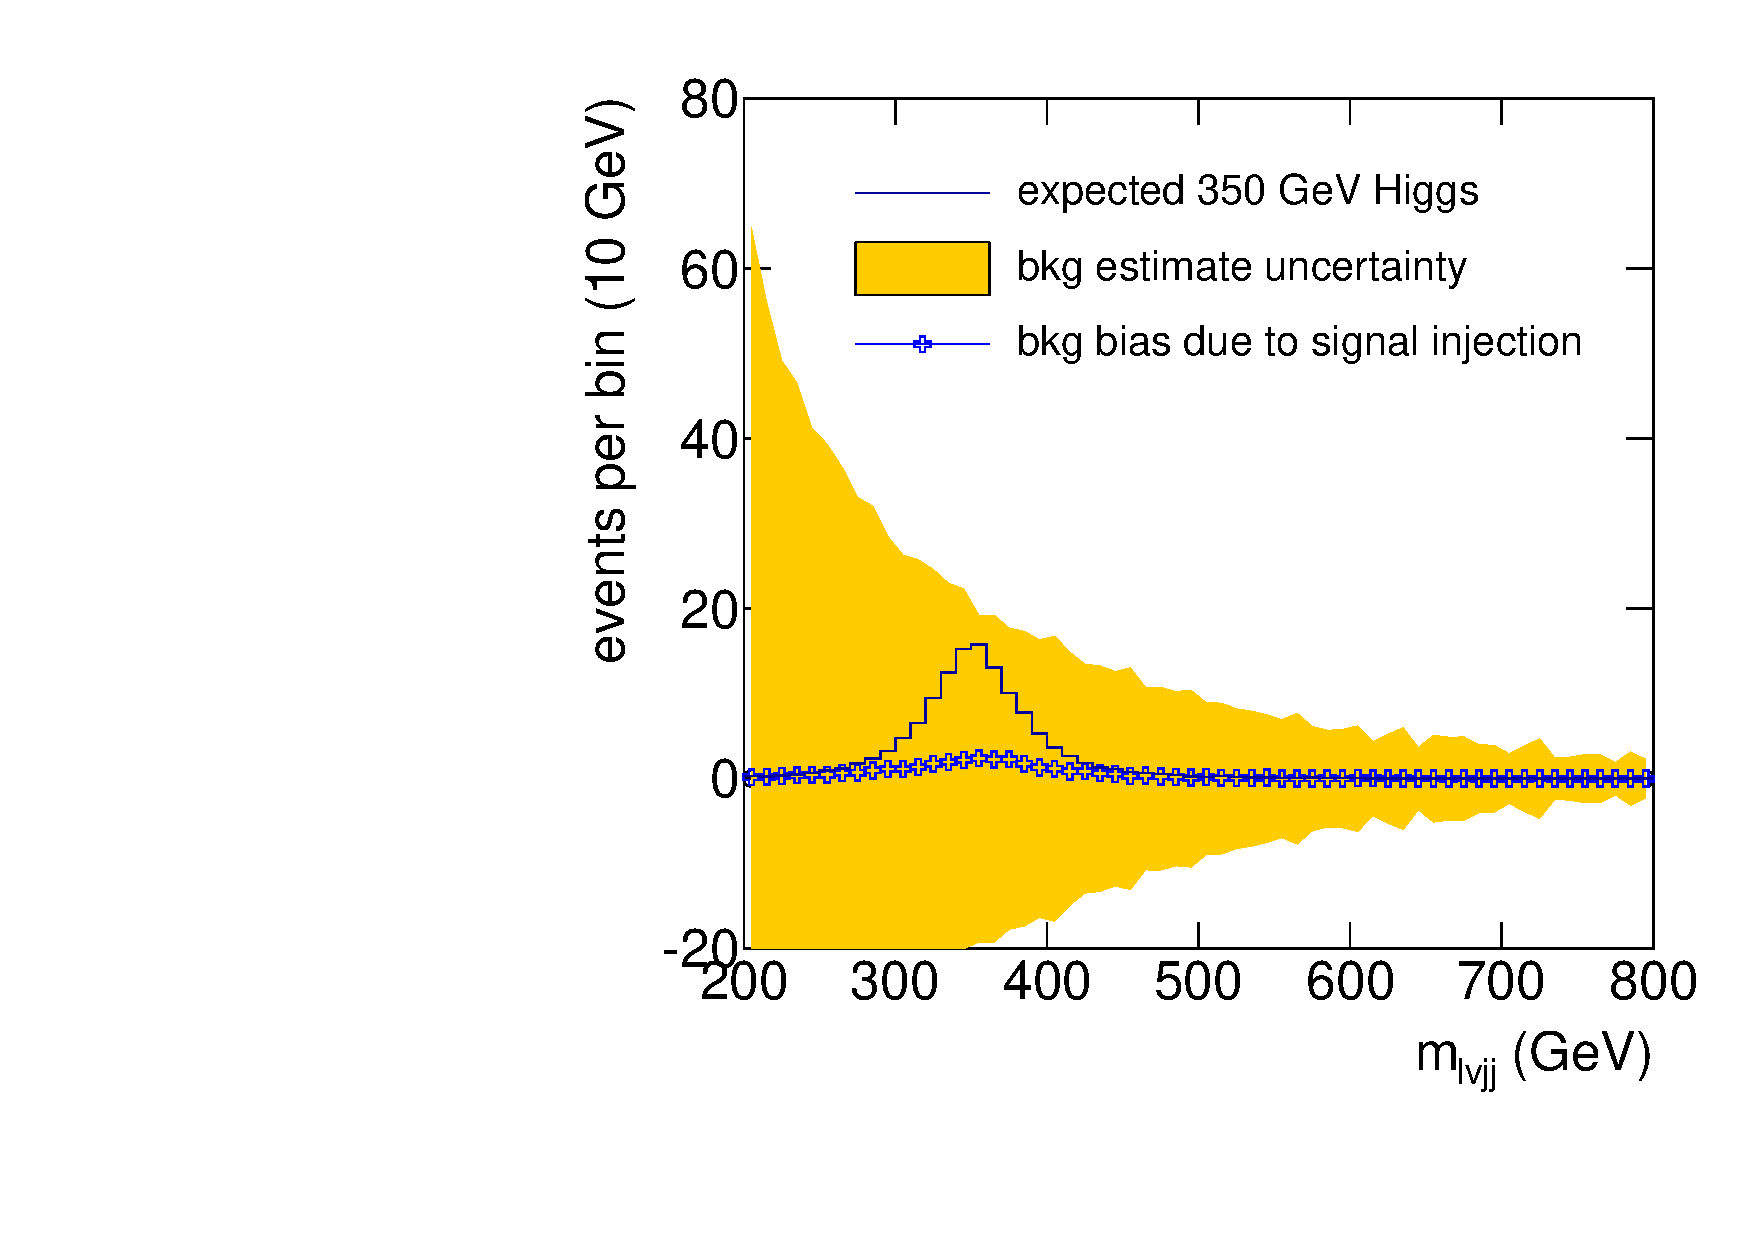
\includegraphics[width=0.45\textwidth]{plots/sideband/injectionTest.pdf}
    \caption{The signal injection test with a Higgs hypothesis of 350~GeV.
             The yellow band represents the error in the extrapolation without signal injection, 
             the blue crosses show the difference of the backgrounds extarpolated in the two cases,
             and the black line is the expected number of signal events in case of Higgs presence.}
    \label{fig:sbSigInjection}
  \end{center}
\end{figure}
%
As can be seen from the distributions, the signal contamination in the sideband region
induces a negligible effect, both compared to the expected number of signal events 
and to the uncertainty band associated to the background estimate.


% ---- ---- ---- ---- ---- ---- ---- ---- ---- ---- ---- ---- ---- ---- ---- ---- ---- ---- ---- ---- ---- ---- ----


\subsection{Analysis results}


The analysis procedure is therefore applied to the signal box.
Figure~\ref{fig:sbSignalBox} shows the four-body mass spectrum in the signal region (black dots)
superimposed to the exapolated background (yellow band) on the left,
and the ratio of the two on the right.
The bars on data represent the statistical uncertainty, 
while the uncertainty bands is due to the statistics in the sideband
summed in quadrature to the systematics of the extrapolation factor.
%
\begin{figure}[htb]
  \begin{center}
    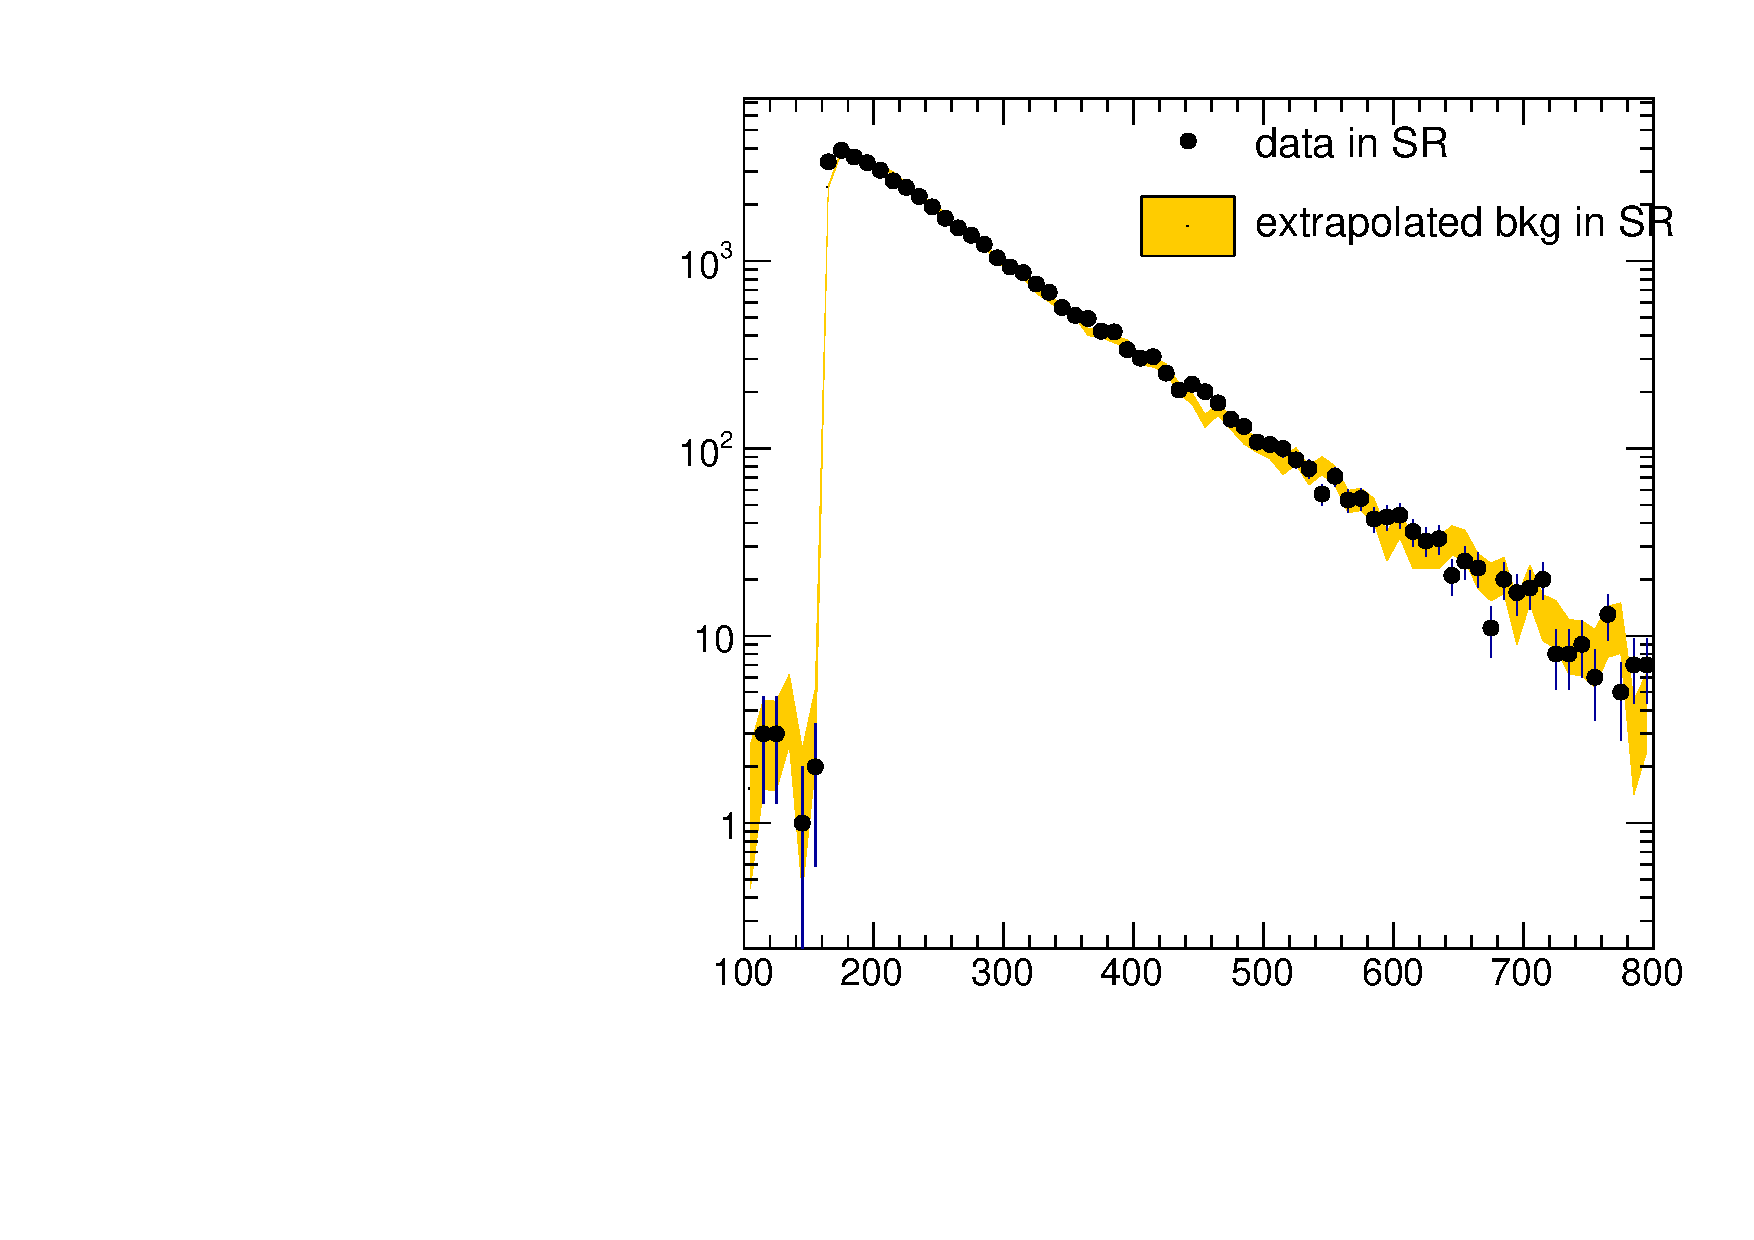
\includegraphics[width=0.45\textwidth]{plots/sideband/sbDATADistrib.pdf}
    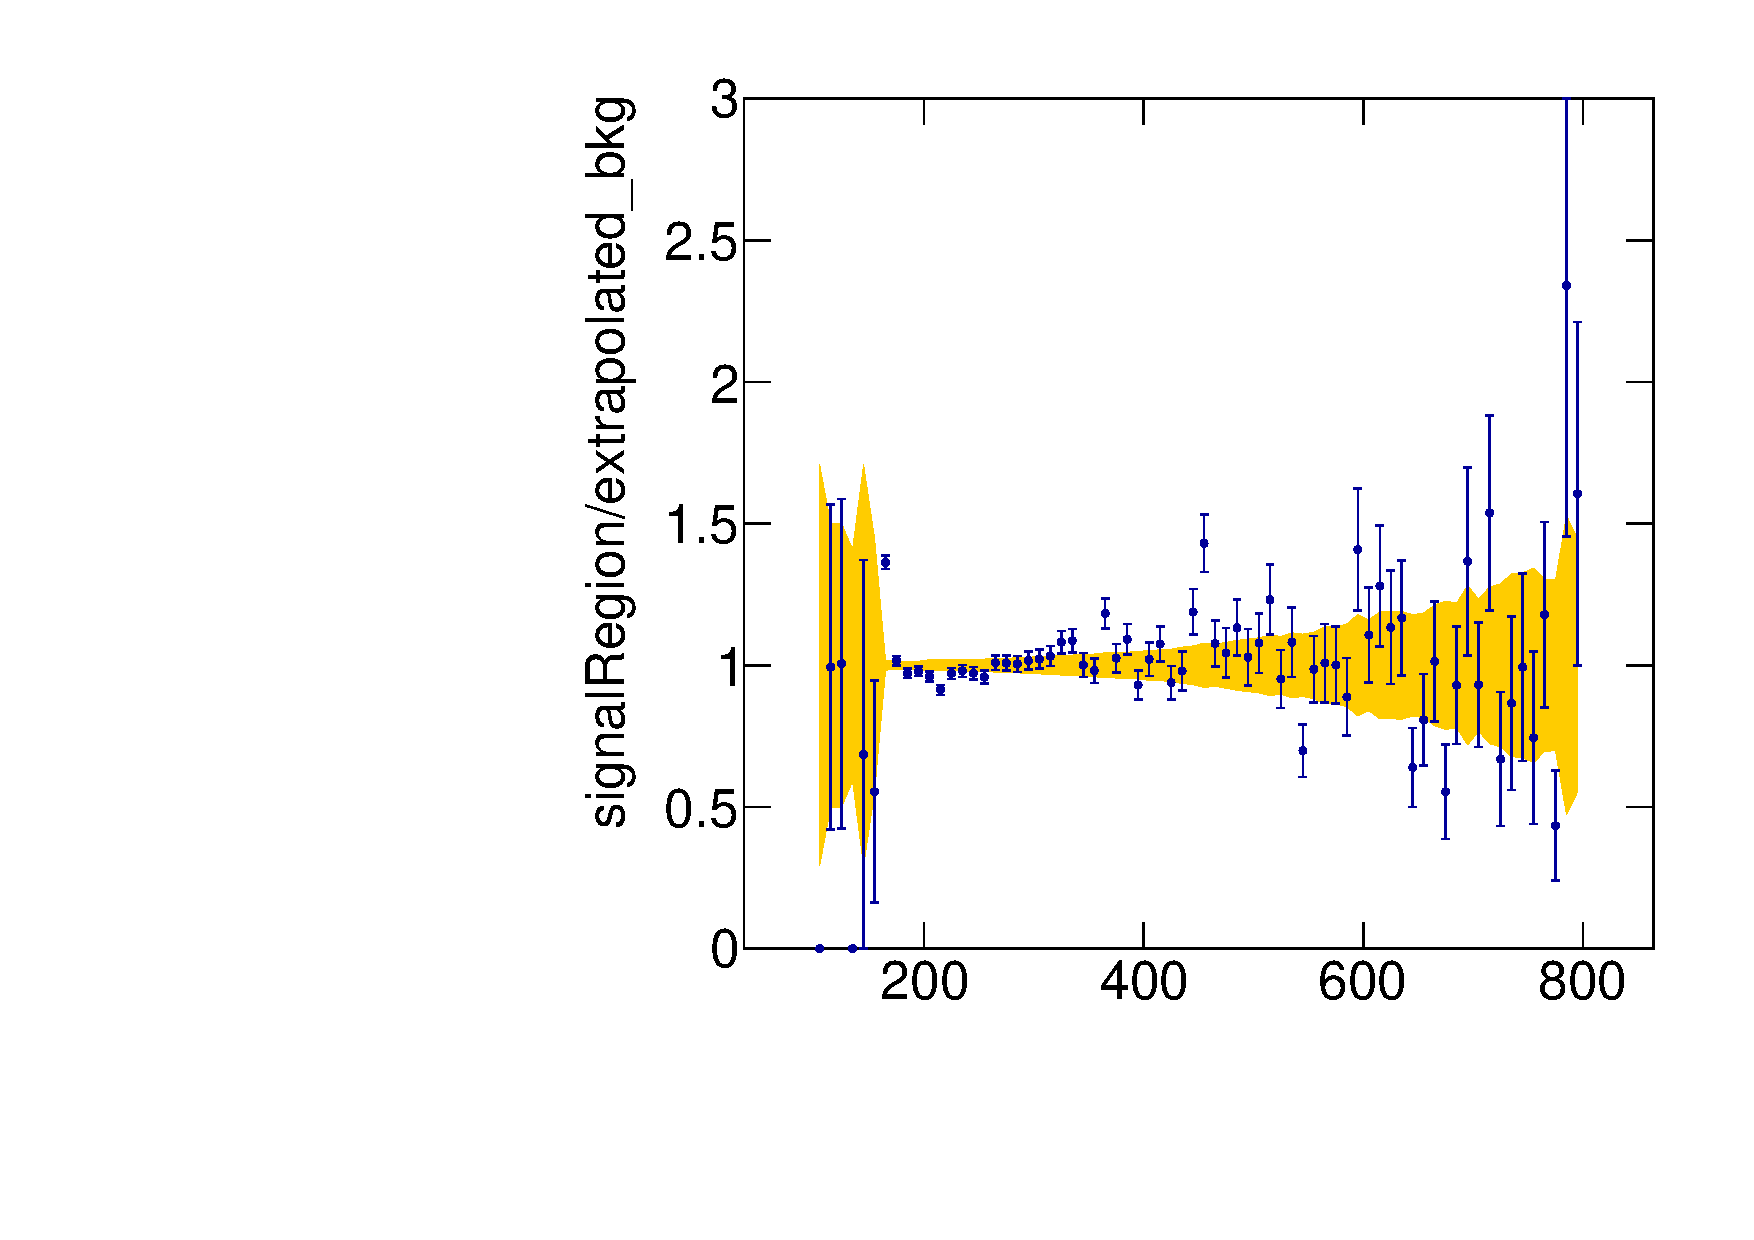
\includegraphics[width=0.45\textwidth]{plots/sideband/sbDATAPull.pdf}
    \caption{the four-body mass spectrum in the signal region (black dots)
             superimposed to the exapolated background (yellow band) on the left,
             and the ratio of the two on the right.
             The bars on data represent the statistical uncertainty, 
             while the uncertainty bands is due to the statistics in the sideband
             summed in quadrature to the systematics of the extrapolation factor.}
    \label{fig:sbSignalBox}
  \end{center}
\end{figure}
%
and Table~\ref{tab:sbEventCounts} shows the number of events measured in the signal region,
the number of expected backgrounds as extrapolated from the sidebands
and the number of Higgs events expected for each mass hypothesis,
within the windows listed in Table~\{tab:fitMHWindows}.
%
\begin{table}[htb]
  \begin{center}
  \begin{tabular}{c|c|c|c}
  \hline 
  Higgs mass (GeV)  &  extrapolated background  &  measured events & expected signal \\
  \hline
  250               &   10061 $\pm$ 95          &     9829         &                 \\
  300               &    6056 $\pm$ 71          &     6194         &                 \\
  350               &    4465 $\pm$ 61          &     4717         &                 \\
  400               &    3159 $\pm$ 51          &     3254         &                 \\
  450               &    2367 $\pm$ 45          &     2489         &                 \\
  500               &    2159 $\pm$ 44          &     2295         &                 \\
  550               &    1077 $\pm$ 32          &     1116         &                 \\
  600               &    1089 $\pm$ 32          &     1120         &                 \\
  \hline
  \end{tabular}
  \end{center}
  \caption{For each Higgs mass hypothesis,
           the number of extrapolated background events 
           obtained with the $m_{jj}$ sideband extrapolation fit, 
           the number of measured events, 
           the number of expected Higgs events 
           in the mass windows of Table~\ref{tab:fitMHWindows}
           are reported.}
  \label{tab:fitResults}
\end{table}
%



% original output from the code, the expected signal is for mH 350 GeV always
% mass : (min,max) : total : bkg_count +- bkg_count_error | expSignal : bkg_count : bkg_count_error / bkg_count : total : 
% MH | 250 : (220,270) : 9829 : 10060.7 +- 94.9274 | 3.69268 : 10060.7 : 0.00943545 : 9829 : 
% MH | 300 : (270,330) : 6194 : 6055.83 +- 71.4637 | 28.2232 : 6055.83 : 0.0118008 : 6194 : 
% MH | 350 : (310,390) : 4717 : 4465.07 +- 60.8026 | 90.5369 : 4465.07 : 0.0136174 : 4717 : 
% MH | 400 : (350,440) : 3254 : 3159.38 +- 51.3834 | 61.5256 : 3159.38 : 0.0162638 : 3254 : 
% MH | 450 : (390,510) : 2489 : 2366.92 +- 45.2027 | 18.8315 : 2366.92 : 0.0190976 : 2489 : 
% MH | 500 : (410,570) : 2295 : 2158.84 +- 43.8574 | 10.7613 : 2158.84 : 0.0203153 : 2295 : 
% MH | 550 : (470,610) : 1116 : 1077.32 +- 31.8663 | 2.69835 : 1077.32 : 0.0295793 : 1116 : 
% MH | 600 : (480,660) : 1120 : 1088.73 +- 32.3364 | 2.25134 : 1088.73 : 0.029701 : 1120 : 



% ---- ---- ---- ---- ---- ---- ---- ---- ---- ---- ---- ---- ---- ---- ---- ---- ---- ---- ---- ---- ---- ---- ----


\subsection{Systematic uncertainties}


% ---- ---- ---- ---- ---- ---- ---- ---- ---- ---- ---- ---- ---- ---- ---- ---- ---- ---- ---- ---- ---- ---- ----


\subsection{Limit extraction}


